% PlanArena, Computational Urban Science version (anonymised for double-blind review). Filled from results/ by
% planarena/paper.py (python -I -m planarena.paper), like paper/paper.tex.in. Do not edit manuscript.tex.
% Author details and the full declarations are on the separate title page (title_page.tex.in).
\documentclass[10pt]{article}
\usepackage[a4paper,margin=25mm]{geometry}
\usepackage{fontspec}
\setmainfont{texgyretermes}[Extension=.otf, UprightFont=*-regular, BoldFont=*-bold,
  ItalicFont=*-italic, BoldItalicFont=*-bolditalic]
\usepackage{microtype}
\usepackage{booktabs}
\usepackage{graphicx}
\usepackage{amsmath}
\usepackage{placeins}
\usepackage[authoryear,round]{natbib}
\usepackage[hidelinks]{hyperref}
\usepackage{xurl}
\usepackage{caption}
\captionsetup{font=footnotesize,labelfont=bf,skip=3pt,labelsep=space}
\captionsetup[figure]{name=Fig.}
\usepackage{enumitem}
\setlist{nosep,leftmargin=*}
\usepackage{lineno}
\linenumbers
\setlength{\parskip}{0.2em}
\setlength{\emergencystretch}{1.5em}
\renewcommand{\bibfont}{\small}
\graphicspath{{figures/}}

\title{\large\textbf{PlanArena: an integrated land-use optimizer with empirical evaluation}}
\author{}
\date{}

\begin{document}
\maketitle
\vspace{-3em}

\begin{abstract}
\noindent Deciding which land uses go where is a location-allocation problem with multidimensional effects: a change
alters homes, jobs, access to services, the tax base, emissions and runoff, interacts with neighbouring parcels, and
may never be built. US cities decide such changes at public hearings, where residents testify but do not vote.
PlanArena is an open land-use optimizer that measures these effects and represents stakeholder interests as votes. It
scores any parcel-level change on 11 indicators with sensitivity ranges in 46 ms
(Manhattan) to 0.58 s (New York City), estimates how likely a change is, recommends plans within zoning and
precedent, and compares nine voting rules over simulated stakeholders, on official data for 4{,}995{,}208 parcels
in ten US cities. On held-out Manhattan lots, given what was built, predicted changes correlated with recorded homes
($r = 0.79$) and emissions ($r = 0.60$), above a gradient-boosted baseline, but overstated total homes
1.47-fold and had no skill for jobs. Redevelopment was ranked out of time with an area under the receiver
operating characteristic curve (AUC) of 0.851--0.902, but observed-to-predicted event ratios ranged 0.07--1.70 across years.
Likelihood weighting brought housing projections from 76--193 to 0.80--2.60 times what was
built; a five-year trend ranked districts better than build-out projections. Searches were checked against exhaustive enumeration; the
votes are illustrative.

\smallskip\noindent\textbf{Keywords:} Land-use optimization $\cdot$ Urban digital twin $\cdot$ Impact assessment
$\cdot$ Planning support systems $\cdot$ Computational social choice $\cdot$ Model validation
\end{abstract}

\section{Introduction}

Deciding which land uses go where (housing, jobs, services, open space) is a location-allocation problem
\citep{church1974,revelle2005}. Its effects are hard to measure for four reasons.
\begin{itemize}
\item \textbf{Many dimensions.} One change alters homes, jobs, access to shops, parks and facilities, the tax base,
energy use and runoff, and these trade off against each other \citep{malczewski2006,rahman2021}.
\item \textbf{Spatial interaction.} Effects spread to neighbouring parcels through walking distance, land-use mix and
competition for development \citep{verburg2004}.
\item \textbf{Uncertainty.} A permitted change may never be built. In three Manhattan rezonings replayed here,
capacity projected 8{,}423 homes on development sites; 561 were built by 2025.
\item \textbf{Competing interests.} Residents, developers, businesses, environmental advocates and city finances weigh
these effects differently, and no single answer is correct \citep{rittel1973}.
\end{itemize}

\paragraph{How decisions are made today.} In US cities, rezonings and plan amendments are decided at public hearings.
\begin{itemize}
\item \textbf{The process.} Planning staff prepare a report, and large rezonings, such as those replayed here, add an
environmental review that projects development on identified sites. Residents and advocates testify; the planning
commission and the council vote.
\item \textbf{Testimony is advisory.} Residents are heard but do not vote. Speakers at planning and zoning meetings are
disproportionately older, male, long-time homeowners \citep{einstein2019}, and legally required hearings meet few
goals of participation \citep{arnstein1969,innes2004,fung2006}.
\item \textbf{Fragmented evidence.} Environmental, fiscal and access effects arrive as separate studies, if at all, and
are rarely weighed together.
\end{itemize}

\paragraph{What computation can measure.} Each part of the problem now has a technical tool:
\begin{itemize}
\item \textbf{parcel-level impact models} calibrated on observed records, which measure many indicators at once;
\item \textbf{supervised learning on parcel histories}, tested out of time, which estimates how likely a change is
\citep{tepe2020,carruthers2024};
\item \textbf{graph neural networks} over parcel adjacency, which represent spatial dependence;
\item \textbf{many-objective evolutionary search} \citep{deb2014}, which explores the combinatorial space of plans;
\item \textbf{computational social choice and bargaining} \citep{nash1950,brandt2016}, which turn stakeholder
preferences into a decision. Game-theoretic simulation has been applied to collective land-use decisions
\citep{abolhasani2022}.
\end{itemize}
Planning support systems (PSS) and urban digital twins aim to combine such tools
\citep{klosterman1999,geertman2020,batty2018,lehtola2022}. Three gaps remain:
\begin{itemize}
\item \textbf{Untested outputs.} Their outputs are seldom tested against outcomes \citep{vonk2005,lei2023,azadi2025,
kruse2026}.
\item \textbf{Optimization.} It rarely asks whether recommended changes are plausible, or how the choice depends on the
decision rule \citep{zheng2023,feng2024,lin2025}.
\item \textbf{Fragmented data.} The data are spread across agencies and schemas, some only as documents:
Philadelphia's land-use plan exists only as maps in 17 PDF district plans.
\end{itemize}

\paragraph{This paper.} PlanArena is an open land-use optimizer that measures the impact of any parcel-level change
and makes stakeholder interests part of the decision. It contributes:
\begin{enumerate}
\item \textbf{Measurement.} Any edit is scored on 11 indicators in three pillars, with sensitivity
ranges, at interactive speed. Each edit also shows what exists, what zoning permits, what the plan intends and how
likely the change is.
\item \textbf{Optimization and decision.} The optimizer recommends plans within zoning and precedent. Resident,
environmental, business, developer and fiscal interests vote on candidate plans under nine rules, and residents also
vote block by block.
\item \textbf{Official data for ten cities.} Existing use, plan and zoning for 4{,}995{,}208 parcels are on one
schema, with a validated method to digitise plans published as vector PDF maps.
\item \textbf{Empirical evaluation where data allow} (Sect.~\ref{sec:validation}): held-out and out-of-time tests of
impacts, likelihood and projections, exhaustive checks of the searches, and the type of evidence behind each claim,
with design guidance drawn from the results.
\end{enumerate}
\textbf{Scope.} Impacts are evaluated in Manhattan only; elsewhere coefficients are national or regional. Zoning is
represented by use permissions and maximum floor-area ratios, access by straight-line distance. Votes rest on assumed
utilities, not elicited preferences, and usability with planners is not evaluated. Online Resource 1 specifies every model and test.

\section{Related work}\label{sec:related}

\paragraph{PSS and urban digital twins.} PSS combine suitability, demand projection and allocation for scenario
planning \citep{klosterman1999,geertman2020}, often in a geodesign workflow linking representation, change, impact
and decision \citep{steinitz2012}. Their limited use and uncertain usefulness are long-standing concerns
\citep{vonk2005,tebrommelstroet2013,pelzer2017}. Digital twins extend them to integrated, updatable city models
\citep{batty2018,batty2024,white2021,lehtola2022,ferrebigorra2022}. Reviews report technical and organisational
barriers \citep{lei2023,wu2025}, and ambitions ahead of demonstrated contributions \citep{azadi2025,luo2025,kruse2026}.
PlanArena attaches a test against observed data to each output.

\paragraph{Optimization and collective decisions.} Location-allocation models site facilities and uses
\citep{church1974,revelle2005}; multicriteria analysis and multi-objective optimization generate and rank land-use
alternatives \citep{malczewski2006,rahman2021}. Recent work uses deep reinforcement learning
\citep{zheng2023} and explicit stakeholder interests \citep{feng2024,lin2025}. Planning problems have no single correct
solution \citep{rittel1973}, so the rule that turns preferences into a choice matters. Bargaining \citep{nash1950} and
voting rules \citep{schulze2011,brandt2016} have different properties, and bargaining has been combined with land
reallocation \citep{hashemi2026}. Simulated votes are not participation \citep{arnstein1969}; PlanArena uses them
only to show how a choice depends on its rule.

\paragraph{Predicting development, and regulation.} Urban change models range from cellular automata
\citep{clarke1997} and statistical site models \citep{landis1998} to behavioural \citep{waddell2002,waddell2003} and
agent-based simulation \citep{parker2003}, with neighbourhood and temporal effects as priorities
\citep{verburg2004,weerasinghe2025}.
\begin{itemize}
\item \textbf{Parcel models} capture existing and historical neighbourhood conditions \citep{tepe2020}, and machine
learning complements econometrics \citep{carruthers2024}.
\item \textbf{Redevelopment} depends on land value relative to the structure \citep{rosenthal1994,dye2007}. In
Chicago, smaller and older buildings with less lot coverage are replaced more often \citep{weber2006,charles2013}.
\item \textbf{Regulation is not exogenous.} Rezoning follows development opportunity \citep{gabbe2018}, studies differ
on upzoning's short-run effect on construction \citep{freemark2020,dong2024,greenaway2023}, and plans are only partly
implemented \citep{talen1996,laurian2004,brody2005,berke2006,loh2011}.
\item \textbf{Regulation in models.} Recent land-change models integrate zoning and planning rules
\citep{hersperger2018,domingo2021,abolhasani2026} but do not test what they add to prediction on held-out history.
\end{itemize}

\paragraph{Validation.} Land-change predictions should be compared with persistence at several resolutions
\citep{pontius2008,pontius2011}, and their transition probabilities validated directly \citep{black2023}. Under
spatial and temporal dependence, random cross-validation overstates skill \citep{roberts2017,ploton2020}, and models
apply only where new data resemble the training data \citep{meyer2021}. Uncertainty from many coefficients is better
assessed by varying them jointly \citep{saltelli2019}.

\section{The system}\label{sec:system}

A parcel twin holds each city's official layers (Figure~\ref{fig:arch}). Four engines answer the planner's questions:
\begin{itemize}
\item the \textbf{impact engine}: what would a change do?
\item the \textbf{likelihood models}: is it likely?
\item the \textbf{optimizer}: what would do better?
\item the \textbf{decision module}: who would choose it, and under which rule?
\end{itemize}
In the Studio, a browser application, a planner paints uses and floor-area ratios on parcels and sees every
indicator, flag and recommendation update (Figure~\ref{fig:studio}).

\begin{figure}[t]
\centering
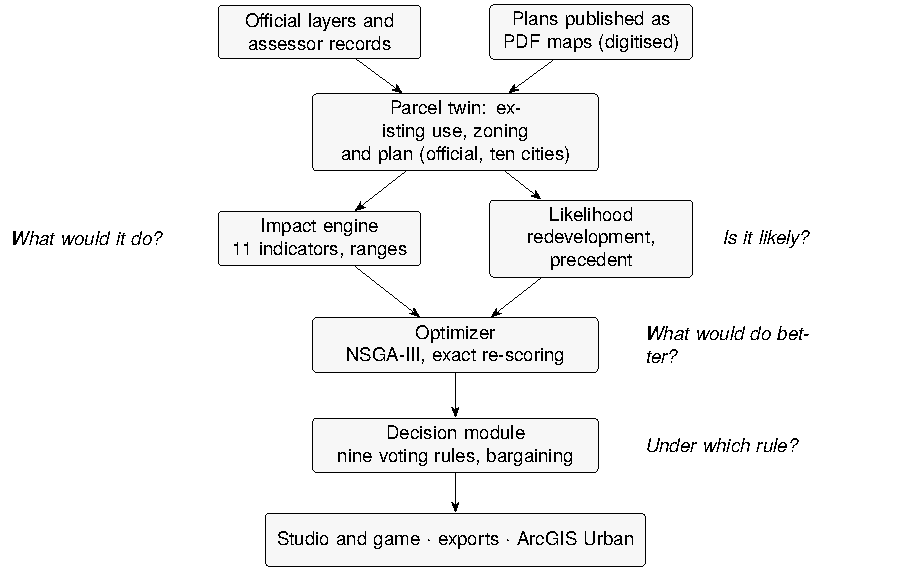
\includegraphics[width=0.72\linewidth]{Fig1}
\caption{Architecture. Every number the system shows comes from one of these components, each with a stated test
(Sect.~\ref{sec:validation})}
\label{fig:arch}
\end{figure}

\begin{figure}[t]
\centering
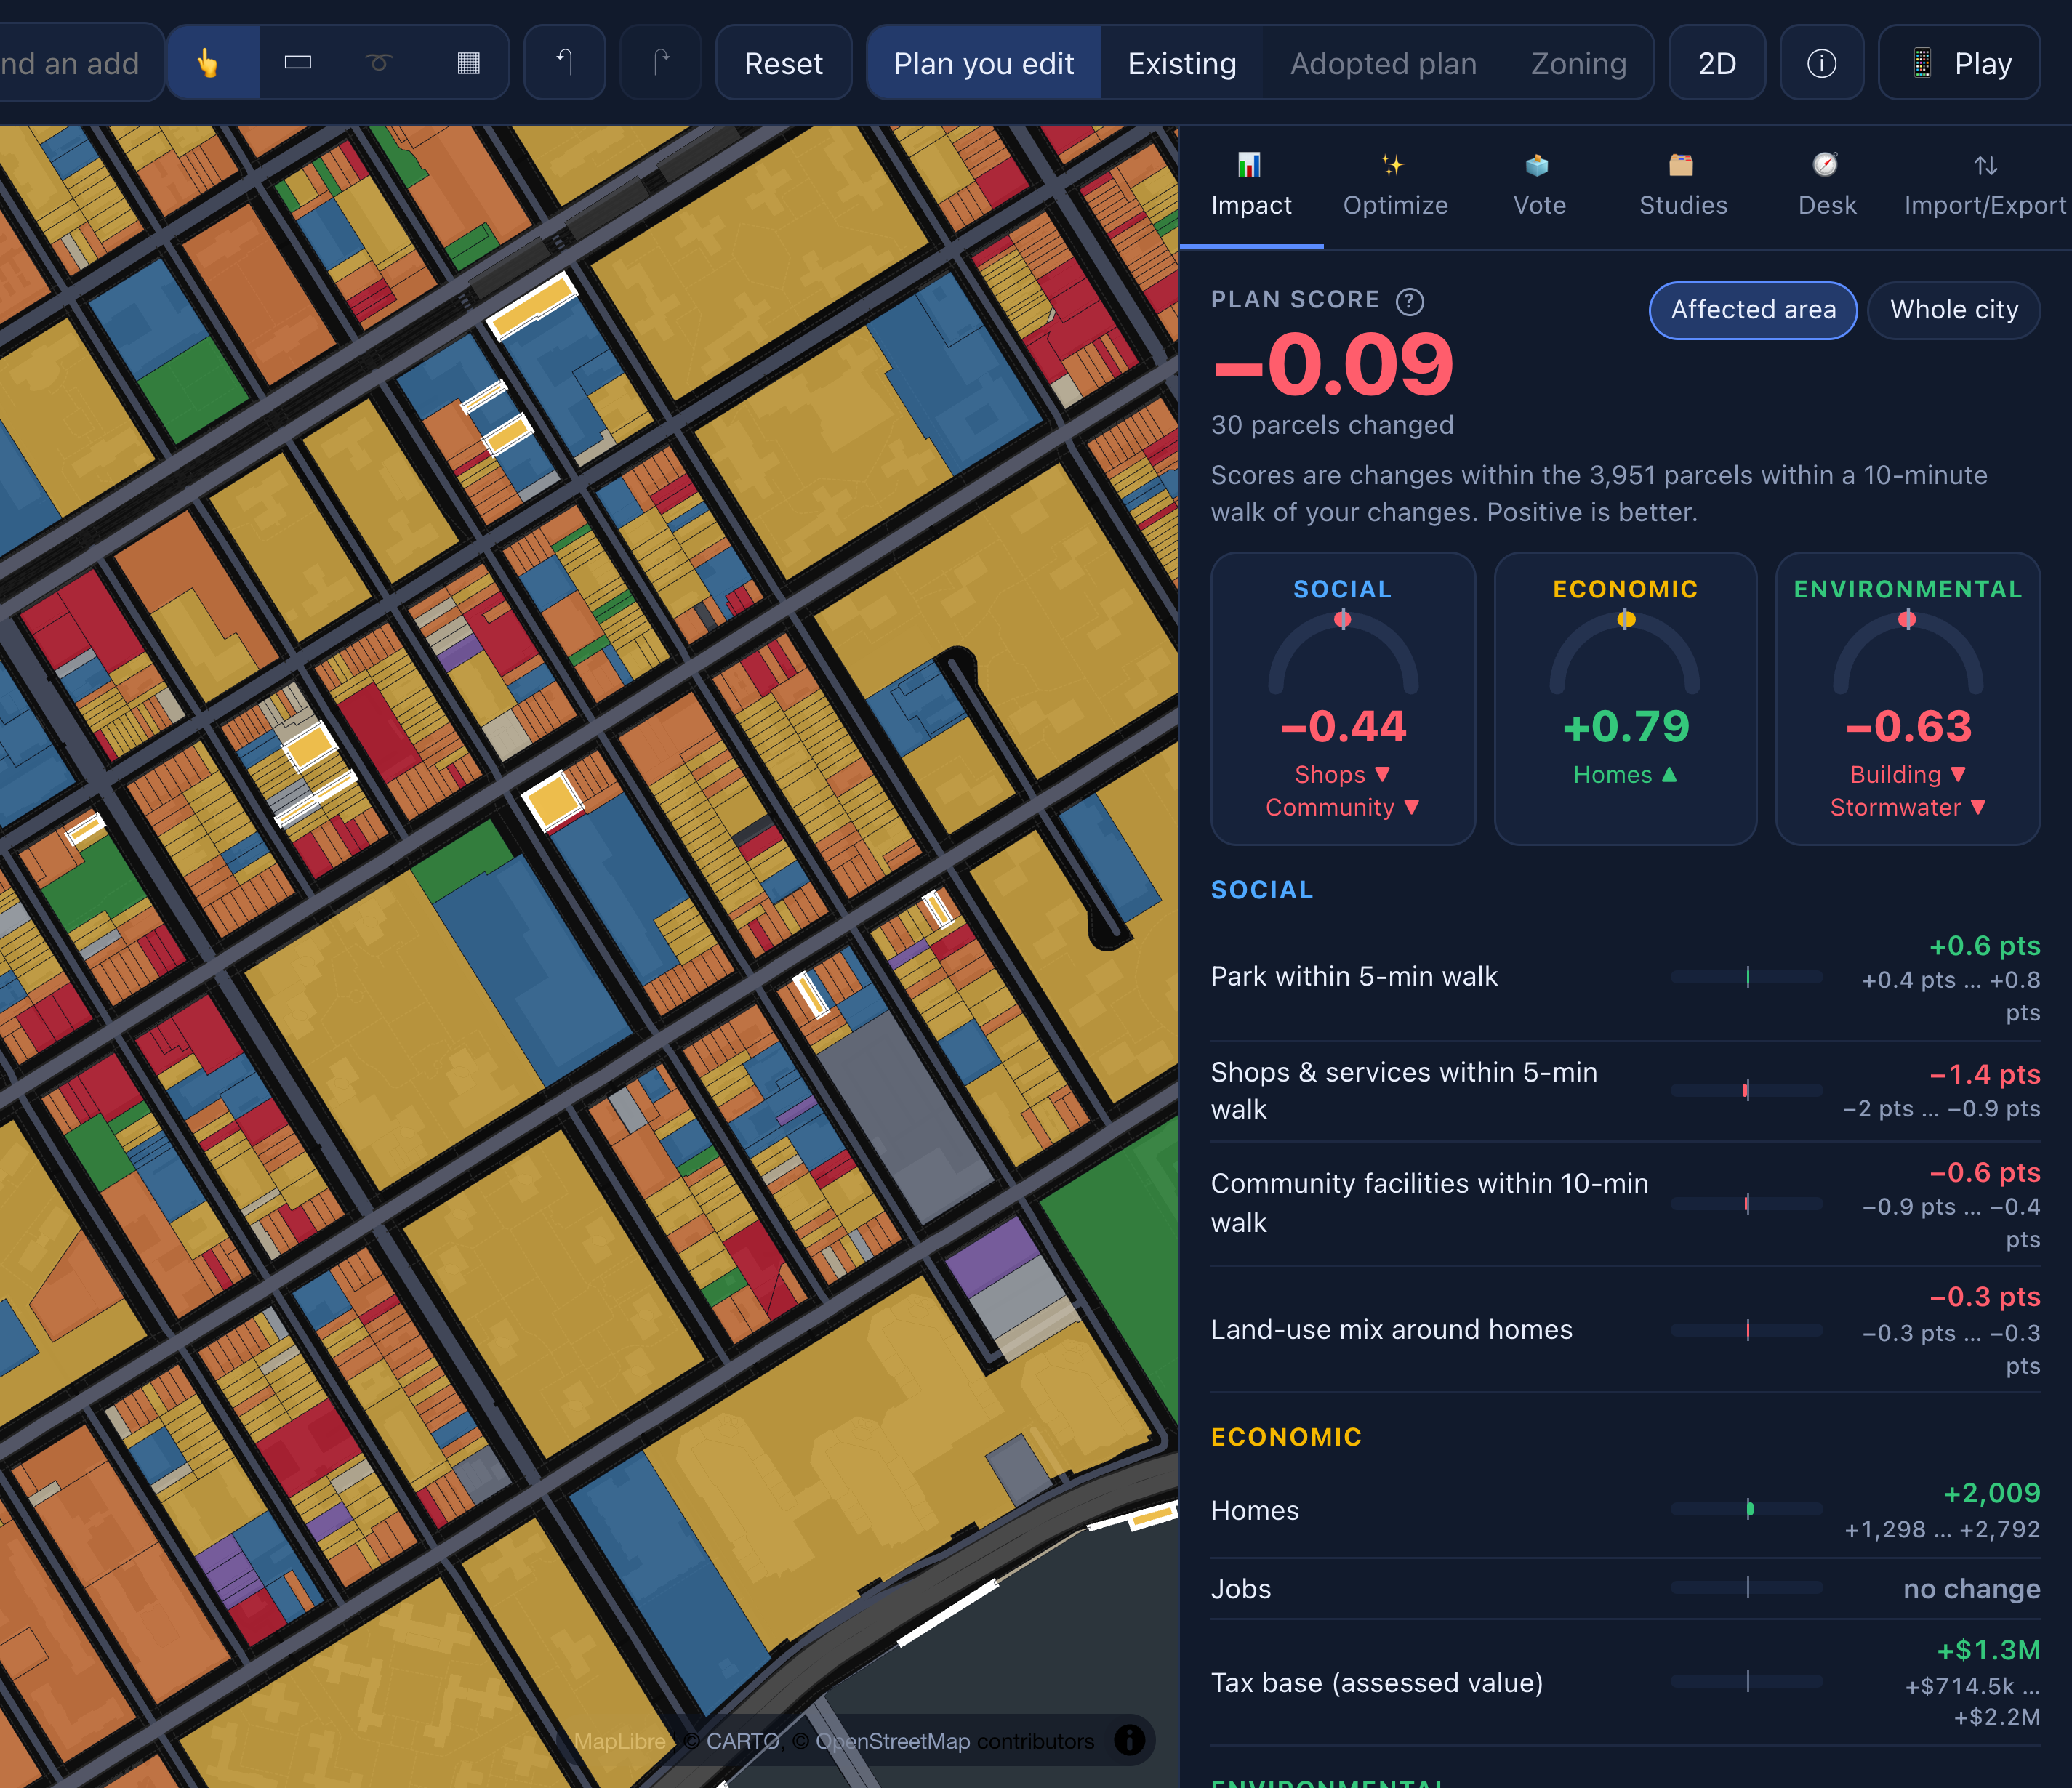
\includegraphics[width=\linewidth]{Fig2}
\caption{The Studio in Manhattan: thirty parking lots and vacant parcels in East Harlem painted as housing
(outlined). Right: plan score, social, economic and environmental pillars, and each indicator's change within a
ten-minute walk with its sensitivity range. Top: switches between the plan being edited and the city's existing,
planned and zoned use. The use palette, left of the map, is not shown}
\label{fig:studio}
\end{figure}

\paragraph{Parcel twin and official layers.} The twin covers the nine largest US cities except San Jose, plus
Milwaukee (Table~\ref{tab:cities}).
\begin{itemize}
\item \textbf{Existing land use} is the parcel land use the city or its regional planning agency publishes, refined
with assessor records where the layer groups uses.
\item \textbf{The adopted plan} (future land use) and \textbf{zoning} are separate layers.
\item \textbf{Classes.} Explicit crosswalks map every source code to 16 classes: three housing types, mixed use,
retail, office, hotel, industry, warehousing, education, health, civic, open space, transportation, parking and
vacant land. The classes nest in nine analysis groups.
\item \textbf{Records.} Floor area, homes, year built and assessed value come from assessor or city records, with
estimated fields flagged. Jobs are fitted to block counts of the Longitudinal Employer--Household Dynamics
(LEHD) programme \citep{data_lodes}.
\item \textbf{Provenance.} Inputs are downloaded by script, with URL and SHA-256 hash recorded.
\item \textbf{Philadelphia's plan}, published only as PDF maps, is digitised (Appendix~\ref{app:digitise}):
15 of 17 plans \citep{data_phila2035}, covering 83\% of parcels, with median
registration errors of 0.3--2.2 m, each checked against a shifted-map control.
\item \textbf{Missing plans.} Where a city publishes no plan as data, the layer is absent, not estimated.
\end{itemize}

\begin{table}[t]
\centering
\scriptsize
\setlength{\tabcolsep}{4pt}
\caption{The ten cities: official parcel layers on one schema. Shares are of the city's parcels.}
\label{tab:cities}
\begin{tabular}{lrllllll}
\toprule
City & Parcels & Existing use (source) & Share & Adopted plan & Share & Zoning & Homes / Census \\
\midrule
New York & 856{,}634 & MapPLUTO (City Planning) & 100\% & none citywide & -- & 100\% & 1.03 \\
Los Angeles & 672{,}444 & SCAG 2020; county assessor & 100\% & General Plan (SCAG 2019) & 100\% & 100\% & 0.99 \\
Chicago & 606{,}894 & CMAP 2023; county assessor & 100\% & none citywide & -- & 96\% & 1.05 \\
Houston & 630{,}525 & City (appraisal codes) & 97\% & none & -- & -- & 0.95 \\
Phoenix & 510{,}871 & County assessor; MAG & 100\% & General Plan & 100\% & 99\% & 0.99 \\
Philadelphia & 547{,}410 & City Planning Commission; OPA & 100\% & district plans (digitised PDF) & 83\% & 100\% & 0.99 \\
San Antonio & 438{,}009 & Bexar Appraisal District & 100\% & adopted area plans & 61\% & 82\% & 0.99 \\
San Diego & 272{,}948 & SANDAG 2025; county assessor & 100\% & General and community plans & 100\% & 94\% & 1.02 \\
Dallas & 311{,}431 & City 2026; DCAD & 100\% & forwardDallas! 2.0 & 99\% & 79\% & 0.98 \\
Milwaukee & 148{,}042 & MPROP & 100\% & PDF only (not included) & -- & 99\% & 1.06 \\
\textit{All} & 4{,}995{,}208 &  &  &  &  &  &  \\
\bottomrule
\end{tabular}
\par\smallskip
\begin{minipage}{0.95\linewidth}\footnotesize Existing use is the city's or regional agency's parcel land use, refined by assessor records where the layer groups uses. Homes / Census: homes in the twin over Census 2020 housing units. Houston has no zoning. Milwaukee's area plans are published as PDFs that could not be downloaded by script. Sources: New York \citep{data_mappluto}; Los Angeles \citep{data_scag}; Chicago \citep{data_cmap}; Houston \citep{data_houston}; Phoenix \citep{data_maricopa}; Philadelphia \citep{data_opa}; San Antonio \citep{data_bexar}; San Diego \citep{data_sandag}; Dallas \citep{data_dallas}; Milwaukee \citep{data_mprop}.\end{minipage}
\end{table}

\paragraph{Impact engine.} An edit sets a parcel's use and, optionally, its floor-area ratio (FAR). The engine
computes the 11 indicators of Table~\ref{tab:indicators} within a ten-minute walk and citywide.
\begin{itemize}
\item \textbf{Unchanged parcels} keep their observed values, so the baseline reproduces the records exactly.
\item \textbf{Changed parcels} follow a hybrid delta rule. A density-only change on a consistent record scales the
observed composition; a use change removes the observed old use and adds the modelled new one (Online Resource 1,
Sect.~S3).
\item \textbf{Derived quantities.} Homes follow from residential floor area and the parcel's floor area per home.
Jobs follow from floor-area components and rates fitted to LEHD counts. Emissions follow from energy intensities and
emission factors derived from New York's benchmarking data (Local Law 84, LL84) and emission limits (Local Law 97)
\citep{data_ll84_2023}.
Runoff follows from surface coefficients, and value from the difference between modelled values.
\item \textbf{Access, mix and green cover} are recomputed on a 50 m raster within straight-line radii of 400 m and
800 m, not along walking routes.
\item \textbf{Ranges.} Every coefficient has a source and a status, and low and high variants give each indicator a
sensitivity range. A range has no probability attached and is not a prediction interval.
\end{itemize}
Indicator scores are per cent changes (totals) or percentage points (shares) against the scope's baseline, clipped to
$\pm 100$; a pillar is the mean of its indicators, and the overall score a weighted mean of pillars with weights the
planner sets. Scoring a 50-parcel edit, ranges included, takes
46 ms on Manhattan's 42{,}075 parcels and 0.58 s on New York City's 856{,}634.
Impacts are computed for the nine analysis groups, for which the coefficients are calibrated and validated.

\begin{table}[t]
\centering
\scriptsize
\setlength{\tabcolsep}{4pt}
\caption{Indicators computed for every edit, and how each is tested (Manhattan).}
\label{tab:indicators}
\begin{tabular}{lllll}
\toprule
Indicator & Pillar & Unit & Better & Test \\
\midrule
Homes & economic & units & higher & held-out change \\
Jobs & economic & jobs & higher & existing; change: no skill \\
Tax base (assessed value) & economic & USD & higher & held-out change \\
Park within 5-min walk & social & \% of residents & higher & not validated \\
Shops \& services within 5-min walk & social & adequacy 0-1 & higher & not validated \\
Community facilities within 10-min walk & social & adequacy 0-1 & higher & not validated \\
Land-use mix around homes & social & index 0-1 & higher & not validated \\
Green \& open space & environmental & ha & higher & direct accounting \\
Stormwater runoff & environmental & impervious-equivalent ha & lower & not validated \\
Building emissions & environmental & tCO2e / yr & lower & existing; held-out change \\
Green cover near homes & environmental & \% of land within 400 m & higher & not validated \\
\bottomrule
\end{tabular}
\par\smallskip
\begin{minipage}{0.95\linewidth}\footnotesize Unchanged parcels keep their observed values; changed parcels follow the delta equations. Each indicator carries a sensitivity range from low and high coefficient variants. Access, mix, green cover and runoff are recomputed from the resulting state but have no observed after-change data to test against. The Studio reports areas in acres (1 acre = 0.405 ha).\end{minipage}
\end{table}

\paragraph{Likelihood, precedent and pattern.} Three models judge plausibility.
\begin{itemize}
\item \textbf{Redevelopment.} A gradient-boosted model (LightGBM), trained only on outcomes known at the decision
year, gives each lot's probability of redevelopment within one, three or five years and its likely new use. Its
inputs are the lot's use, size, built and permitted floor area, age and land share of value, its neighbourhood and its
zoning.
\item \textbf{Precedent.} A conversion is flagged if buildings of that use and size were not converted to the proposed
use in the past decade.
\item \textbf{Pattern.} A graph neural network over parcel adjacency, combined with LightGBM, describes how well a use
fits its surroundings: an existing pattern, not a norm.
\end{itemize}
Edits that depart from the plan or from what zoning allows are flagged (Figure~\ref{fig:inspector}).

\begin{figure}[t]
\centering
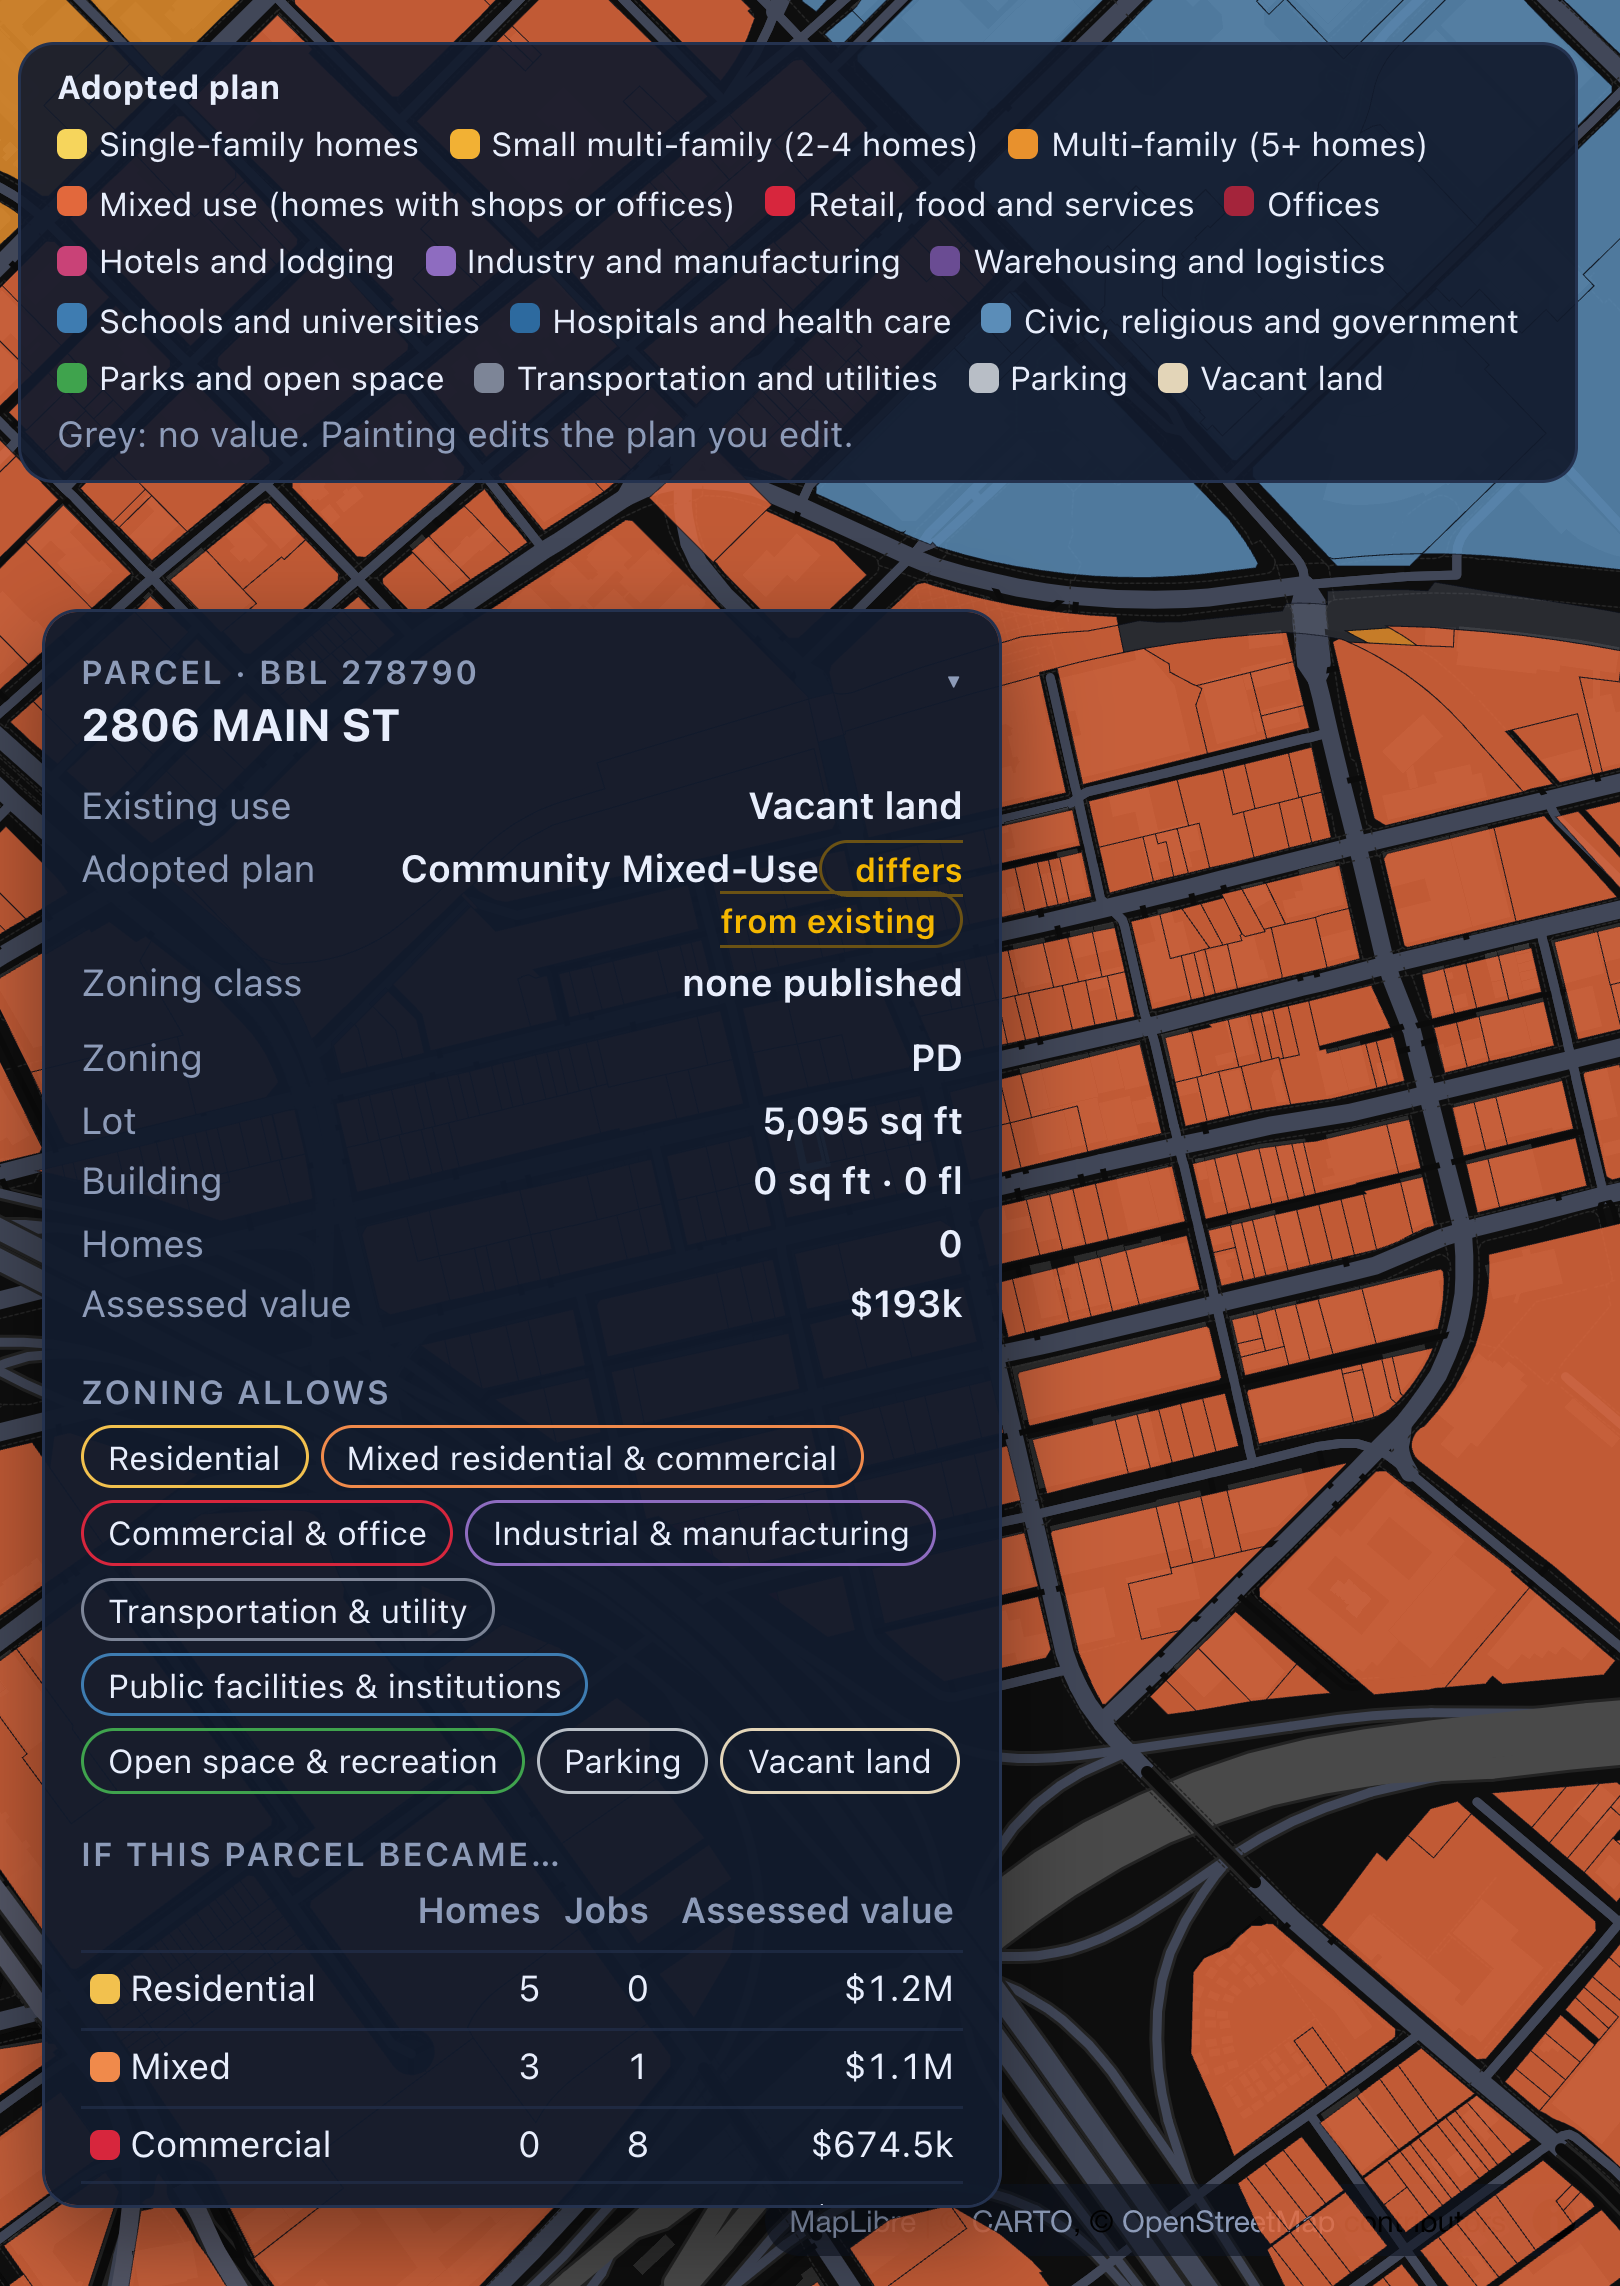
\includegraphics[width=0.62\linewidth]{Fig3}
\caption{Parcel inspector on the adopted-plan layer (Dallas). For a vacant lot the plan designates Community
Mixed-Use, it lists existing use, plan designation (flagged as differing), zoning, the uses zoning allows, and what each
new use would yield in homes, jobs and assessed value}
\label{fig:inspector}
\end{figure}

\paragraph{Optimizer.} The optimizer maximizes the overall score minus a penalty per conversion, under a budget of
changes. The uses zoning permits are a hard constraint, existing homes and protected sites are kept, conversions
without precedent are skipped, and candidates can be restricted to the parcels most likely to be redeveloped. Two
searches are offered:
\begin{itemize}
\item iterated best response over first-order move estimates, with exact re-scoring of the best moves;
\item NSGA-III \citep{deb2014}, which returns a Pareto set across the three pillars, re-scored exactly.
\end{itemize}
Both report the best plan found, not a proven optimum (Online Resource 1, Sect.~S6).

\paragraph{Decision module.} Choices are contested \citep{rittel1973}, so the module shows how the chosen plan depends
on the decision rule.
\begin{itemize}
\item \textbf{Agents.} Five stakeholder agents (residents, business, developers, environmental and city-finance
interests) score candidates from assumed utilities over the indicators.
\item \textbf{Rules.} Nine voting rules are compared with the Nash bargaining solution \citep{nash1950} and a
residents' referendum by block. Schulze's method \citep{schulze2011} decides.
\item \textbf{Reports.} Whether a Condorcet winner exists, whether one insincere ballot could change the outcome, and
the winner's robustness to coefficients and seats.
\end{itemize}
Unlike hearing testimony, these interests are votes: each agent holds one seat on a simulated council, and
residents also vote block by block. The agents stand for interests, not for people, and one agent per interest does
not capture the variety within it. Utilities are editable assumptions, and the output is a simulated scenario, not
public support \citep{arnstein1969} (Figure~\ref{fig:optvote}).

\begin{figure}[t]
\centering
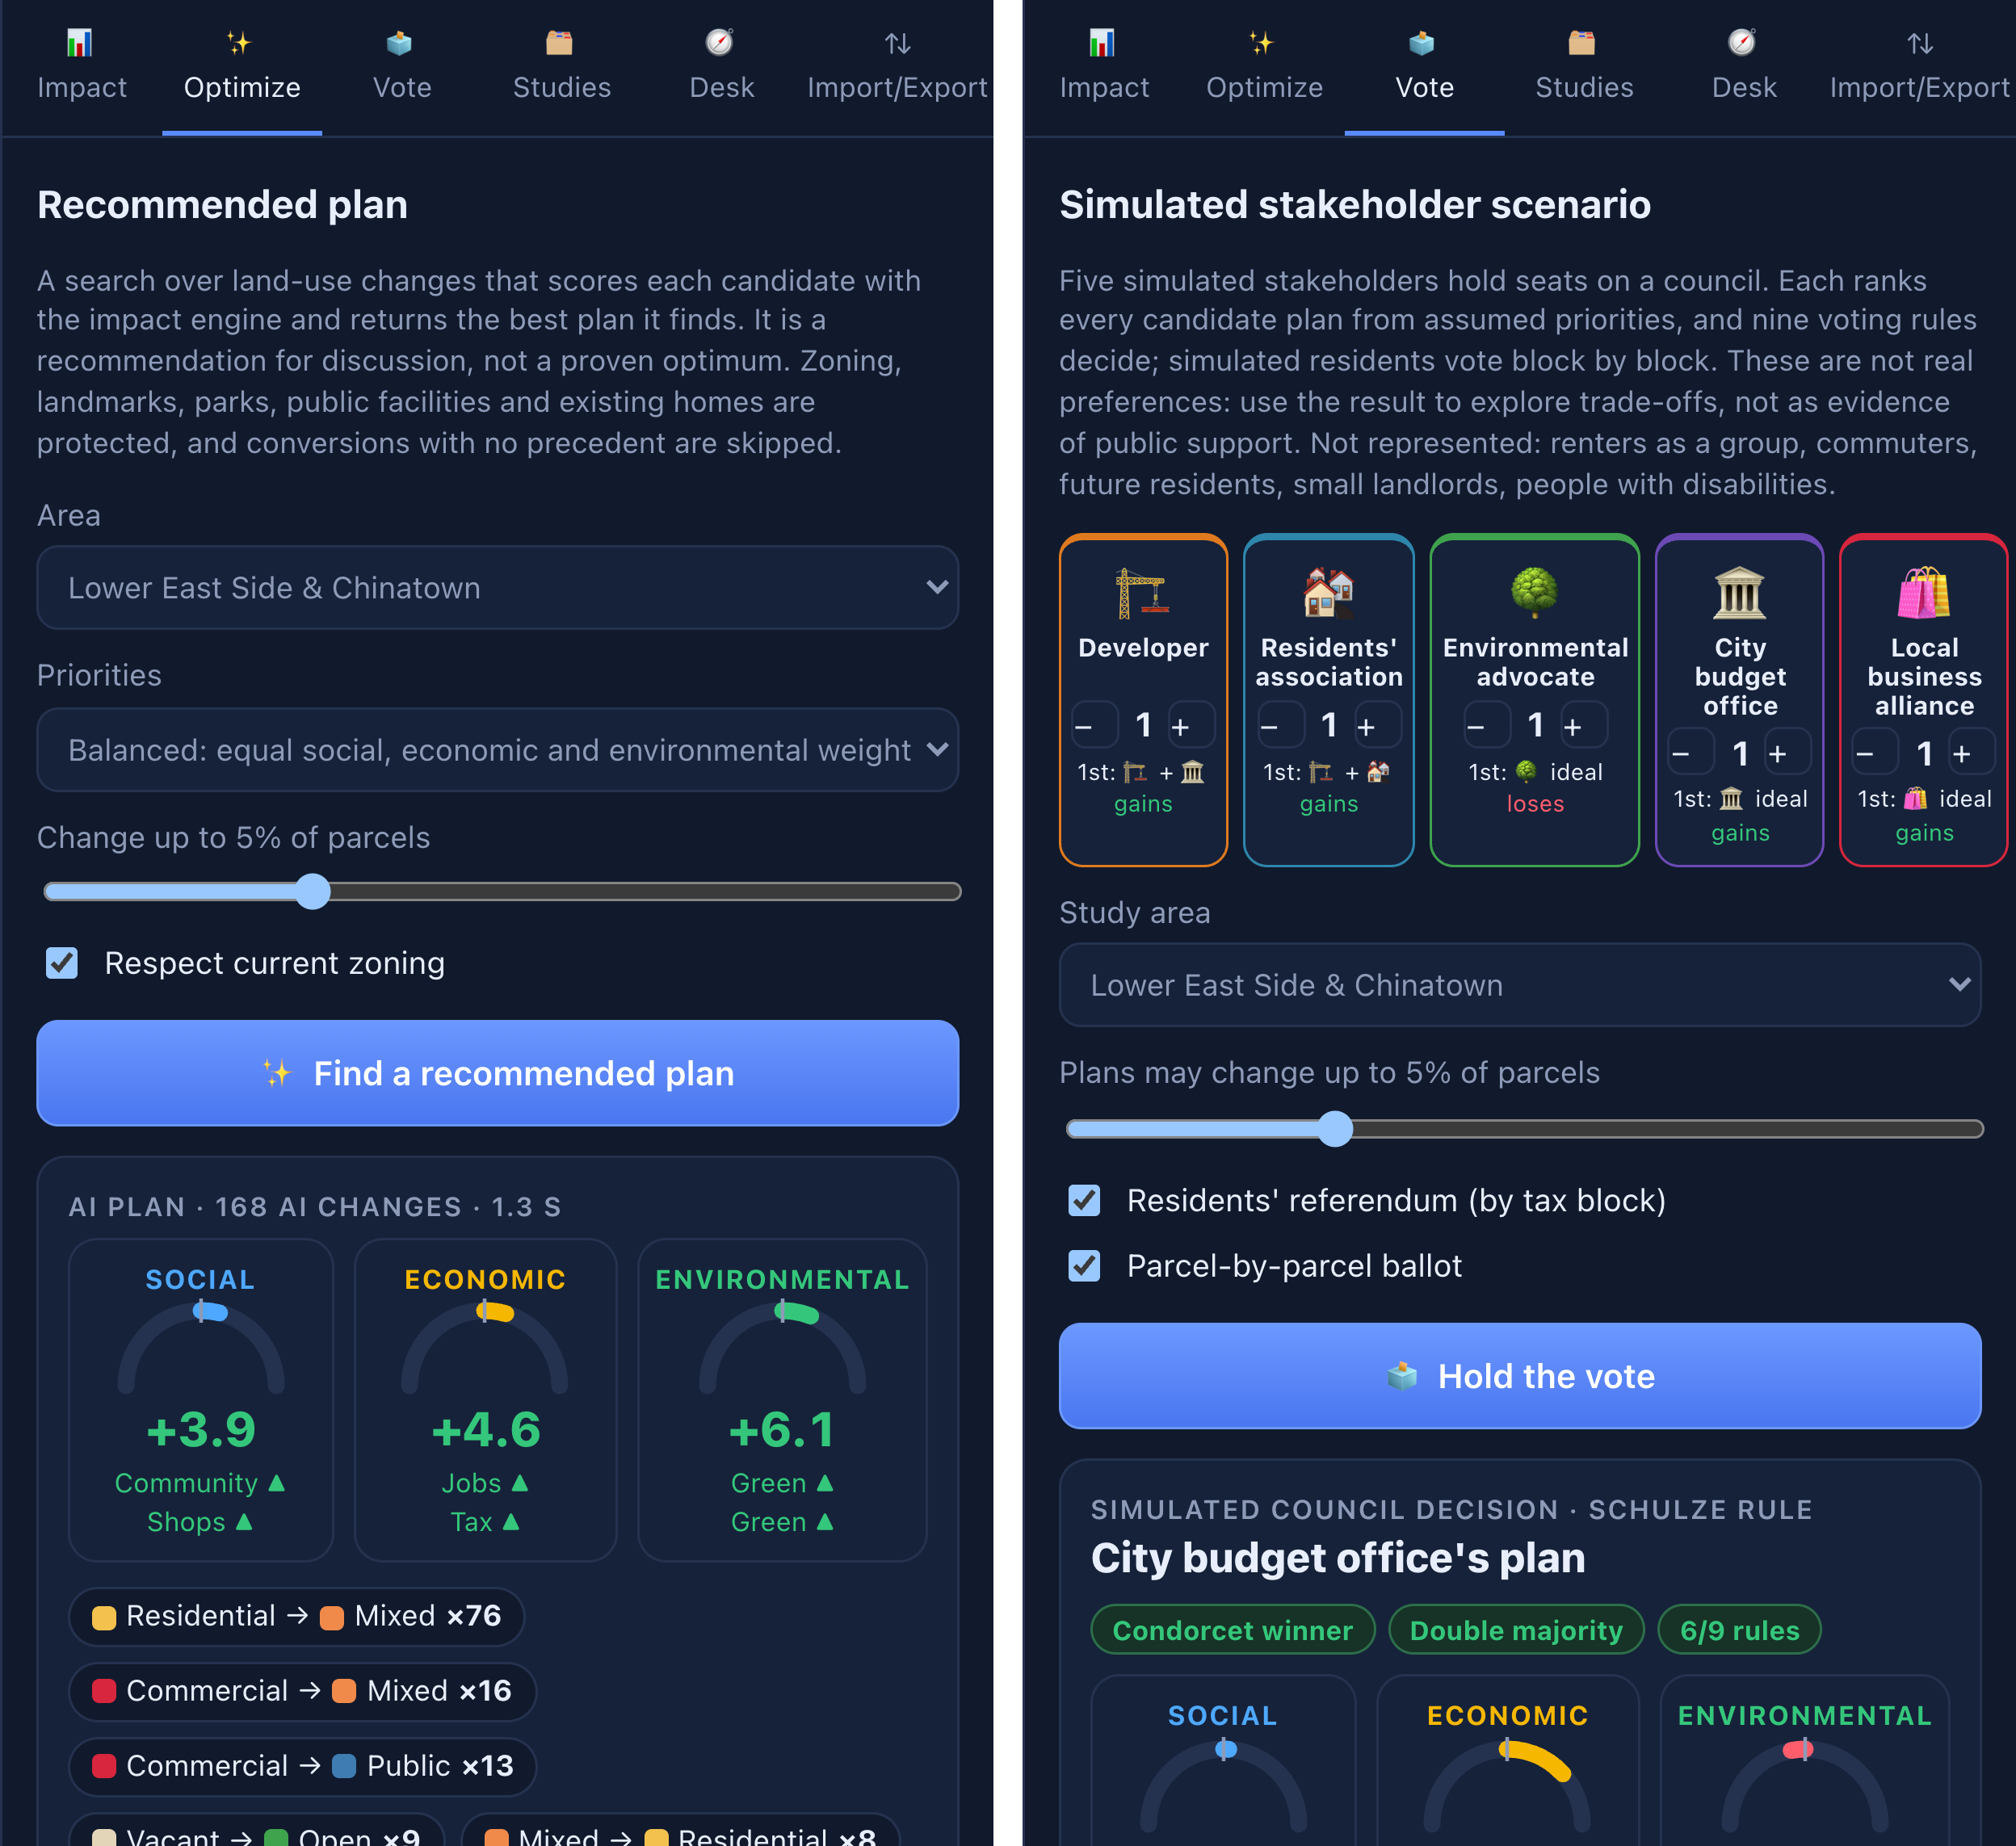
\includegraphics[width=\linewidth]{Fig4}
\caption{Optimizer and decision module for one Manhattan district. Left: the recommended plan, its change in each
pillar and its conversions. Right: the simulated council's decision under Schulze's rule, whether the winner is a
Condorcet winner with a double majority, and how many of the nine rules it wins}
\label{fig:optvote}
\end{figure}

\paragraph{Interface.} Planners can edit parcels by click, box, lasso or search, or upload plans as tables or GIS
files, which are reviewed before they are applied. Studies are stored with a hash-chained audit log. Exports include a
staff-report draft, CSV and GeoJSON files, and the provenance of every coefficient. A phone version presents the engine
as a game. Any city or district exports to ArcGIS Urban: space-use, zoning and land-use types, boundaries, and parcels
with a PlanArena scenario. An online demonstration of the Studio for Manhattan is at \url{https://planarena-manhattan.onrender.com} and the game at
\url{https://planarena-manhattan.onrender.com/play} (an earlier release, v1.0.0-rc.1; the first load can take about a minute); the code for all
ten cities is in the repository (Statements and Declarations).

\section{Evaluation methods}\label{sec:validation}

The claims rest on four kinds of evidence (Table~\ref{tab:design}): \emph{empirical predictive tests}, in which a
prediction made with earlier information is compared with a later outcome on observations not used to build or select
the model; \emph{accounting checks}, in which the twin reproduces records it was built from; \emph{algorithmic
verification} of the searches against exhaustive enumeration; and \emph{illustrative simulation} for the decision
module, which has no observed counterpart.
\begin{itemize}
\item \textbf{Time.} Predictions are trained on one period and tested on a later one; uncertainty comes from
resampling spatial tiles \citep{kunsch1989}, never from random splits \citep{roberts2017}. The cross-city test uses
seven cities with parcel histories (Table S12 in Online Resource 1).
\item \textbf{Development} is defined as each source records it: a new building or large floor-area increase (Los
Angeles, Dallas, New York), a new building (Milwaukee), a change of use class between land-use inventories (Phoenix,
San Diego), or a new-construction permit (Chicago). A building already on the starting record is never counted as new.
\item \textbf{Blocks.} Four feature blocks are added in turn: existing conditions (E), context within 400 m (C),
zoning (Z) and plan (P).
\item \textbf{Leakage control.} Every feature family is dated against the decision year (Online Resource 1,
Sect.~S2). Where a current
zoning or plan layer has dated changes, a conservative variant drops lots whose zoning or plan dates from the window's
start or later; lots that merge or split are followed by their representative point.
\item \textbf{Data.} Manhattan tests use the annual MapPLUTO releases \citep{data_mappluto}, LL84 benchmarking
\citep{data_ll84_2015,data_ll84_2023} and LEHD job counts \citep{data_lodes}; the city panels use the sources of
Table~\ref{tab:cities}.
\end{itemize}

\paragraph{Use of AI tools.} Claude (Anthropic), used through Claude Code, assisted in writing and testing the code,
running the analyses, and drafting the text and Online Resource 1. The author designed the study and the system,
reviewed the code, results and text, read the cited sources and is accountable for the content. Every reference was
checked against the record its DOI or ISBN resolves to. No AI system generated data or results: every number is computed
by the released code from the public inputs, and tests fail if a reported number differs from the result files.

\begin{table}[t]
\centering
\scriptsize
\setlength{\tabcolsep}{4pt}
\caption{Evaluation design: each component, its question, data and type of evidence.}
\label{tab:design}
\begin{tabular}{lp{5.0cm}p{4.0cm}ll}
\toprule
Component & Question & Data & Evidence & Section \\
\midrule
Existing conditions & Does the twin reproduce what is there? & LL84 energy, LEHD jobs, recorded homes & accounting & \ref{sec:r-existing} \\
Planning calculations & Does it reproduce a review's projection from the review's own inputs? & Environmental impact statements (two rezonings) & accounting & \ref{sec:r-existing} \\
Effects of change & Given an observed change, does it predict the effect? & MapPLUTO 2015 vs 2025, held-out folds & empirical & \ref{sec:r-change} \\
Likelihood & Does it rank lots that redevelop, and how many, forward in time? & Rolling origins 2016--2025 & empirical & \ref{sec:r-likely} \\
Official layers & What do zoning and plans add, in other cities? & Seven city panels & empirical & \ref{sec:r-layers} \\
Housing projections & Are projected homes close to what was built? & Four cities; three rezonings & empirical & \ref{sec:r-homes} \\
Optimizer & How close is the best plan found to the best plan? & Exhaustive search; 12 districts & algorithmic & \ref{sec:r-opt} \\
Pareto explorer & Does NSGA-III find the trade-off front? & Exhaustive enumeration of blocks & algorithmic & \ref{sec:r-opt} \\
Realism & Are recommended changes plausible? & 2020 plans vs 2025 outcomes & empirical & \ref{sec:r-opt} \\
Decision module & How does the choice depend on rule, seats and candidates? & Assumed utilities & illustrative & \ref{sec:r-dec} \\
\bottomrule
\end{tabular}
\end{table}

\section{Results}\label{sec:results}

\subsection{Existing conditions and planning calculations}\label{sec:r-existing}

The twin reproduces Manhattan's existing conditions
(accounting checks).
\begin{itemize}
\item \textbf{Emissions.} Modelled emissions match 6{,}234 benchmarked buildings in a year not used for fitting
(log--log $r = 0.807$, median error 31\%, total 1.04 times metered).
\item \textbf{Jobs} correlate with LEHD counts at tract level ($r = 0.843$) and block level ($r =
0.727$).
\item \textbf{Homes.} Given observed use and floor area, homes on 295 lots developed in 2015--2025 total
1.04 times the recorded count ($r = 0.903$).
\item \textbf{Environmental reviews.} Given two rezonings' final environmental impact statements (FEIS) and their own
sites, floor area and uses \citep{data_feis_eh,data_feis_sn}, PlanArena reproduces their projected homes at
0.86 and 1.00 times the review figures.
\end{itemize}

\subsection{Effects of observed change}\label{sec:r-change}

3{,}350 Manhattan lots changed use or floor area substantially between 2015 and 2025. Each was given its 2015
state and its observed new use and floor area, with coefficients from 2015 data. The test is conditional: it checks
the engine given what was built, not whether the change would happen. The delta form, the unit-size rule and a scale
factor were chosen on 1{,}314 lots in two of five spatial folds; results are for the other 2{,}036
(Table~\ref{tab:change}; Online Resource 1, Sect.~S4).
\begin{itemize}
\item \textbf{Homes}: predicted change correlates with recorded change at $r = 0.79$, against
0.68 for gradient-boosted regression and 0.39 for the mean change of the same transition,
both fitted on the selection lots with the same information. The mean absolute error is 12.5 homes per lot,
against 16.5 for predicting no change.
\item \textbf{Value}: $r = 0.74$, against 0.57, but the direction of the change (relative
to the district trend) is right for only 60\% of lots, against 88\% for homes;
\textbf{emissions} of 115 benchmarked buildings: $r = 0.60$, against 0.36.
\item \textbf{Bias.} The engine overstates total homes added 1.47-fold (the regression baseline
1.24-fold). A scale factor fitted on the selection lots brings this to 1.35.
Conversions to mixed use account for 70\% of the excess; commercial-to-mixed conversions alone overstate by
28 homes per lot.
\item \textbf{Jobs.} By census block, predicted job change does not correlate with the change in LEHD counts
($r = 0.05$): the engine has no skill for job change at this scale.
\end{itemize}
Access, mix, green cover and runoff have no after-change data, and the Studio marks them as not validated.

\begin{table}[t]
\centering
\scriptsize
\setlength{\tabcolsep}{3pt}
\caption{Effects of observed change on 2{,}036 held-out Manhattan lots, 2015--2025: given the 2015 state and the observed new use and floor area, predicted against recorded change (Pearson $r$; mean absolute error and mean bias in homes per lot; predicted over observed total).}
\label{tab:change}
\begin{tabular}{lrrrrrrrr}
\toprule
Method & Homes $r$ & MAE & Bias & Total & Value $r$ & Total & Emis.\ $r$ & Total \\
\midrule
PlanArena (deployed form) & 0.79 & 12.5 & 5.6 & 1.47 & 0.74 & 0.70 & 0.60 & 1.24 \\
PlanArena (form chosen on selection lots) & 0.79 & 12.7 & 6.1 & 1.51 & 0.74 & 0.70 & 0.60 & 1.24 \\
\quad $\times$ selection-lot scale & 0.79 & 11.8 & 4.2 & 1.35 & 0.74 & 1.09 & 0.60 & 1.06 \\
Gradient-boosted regression & 0.68 & 15.4 & 2.9 & 1.24 & 0.57 & 1.19 & 0.36 & 1.10 \\
Mean change of the same transition & 0.39 & 22.3 & 1.5 & 1.12 & 0.10 & 1.07 & 0.26 & 2.26 \\
\bottomrule
\end{tabular}
\par\smallskip
\begin{minipage}{0.95\linewidth}\footnotesize Selection lots (1{,}314, two of five spatial folds) chose the form and fitted the baselines and the scale. Predicting no change gives a homes MAE of 16.5. Emissions: 115 benchmarked buildings.\end{minipage}
\end{table}

\subsection{Likelihood of redevelopment}\label{sec:r-likely}

Trained on 2015--2020 outcomes and tested on 2020--2025, the redevelopment model reaches AUC 0.855, against
0.802 for the best simple baseline and 0.833 for a graph neural network, with 26\%
redeveloped among its top 1\% of lots against a base rate of 1.23\%. Across 15 rolling origins
(2016--2025; horizons of one, three and five years), its out-of-time AUC is 0.851--0.902, above the
best baseline at every origin.

\paragraph{Calibration} (Online Resource 1, Sect.~S5). The model ranks lots better than it predicts how many redevelop.
\begin{itemize}
\item \textbf{Totals shift with the cycle.} Observed over predicted redevelopments ranged from 0.07 to
1.70 across origins, and in the seven cities' test windows from 0.42 to 1.60.
\item \textbf{Spread.} Calibration slopes were 0.59--0.95: the probabilities are too spread
out.
\item \textbf{Skill.} Against a constant forecast of the training-period rate, Brier skill was $-$0.97 to
0.15, negative at three of 15 origins.
\item \textbf{Recalibration} on out-of-fold training probabilities corrects the spread (slopes
0.74--1.05) but not the totals, which still range 0.06--1.31
in Manhattan and 0.41--1.24 in the cities: the rate of development changes between
windows in ways a model trained on earlier windows does not anticipate.
\end{itemize}
The probabilities are used to rank sites and to weight projections whose totals are compared with observed rates, not
as forecasts of how many lots will redevelop.

\subsection{What zoning and plans add, across seven cities}\label{sec:r-layers}

Existing conditions alone rank developed lots with out-of-time AUC 0.824--0.911 in six cities, and
0.571 in San Diego, whose one-year window recorded few changes (Table S13 in Online Resource 1;
average precision in Table S15). Adding blocks:
\begin{itemize}
\item \textbf{Context} adds the most: +0.021 to +0.116, significant in five cities
(Table~\ref{tab:gains}, Figure~\ref{fig:gains}). Phoenix is the exception: its land-use series starts in 2022, so
recent change is unknown in its training window.
\item \textbf{Zoning} carries its own signal. Without context, it raises AUC significantly in five of seven cities, and
developed lots were 2.1--9.5 times as likely as others to have a zoning class outside
their existing use group.
\item \textbf{Overlap.} Most of that signal is shared with existing conditions and context: developed lots were also
3.5--19 times as likely to be vacant. Over context, zoning adds a significant gain in
five of seven cities and the plan in three of four, at most +0.021 outside Phoenix.
\item \textbf{Phoenix.} Zoning adds +0.049 and the plan +0.054, and 45\% of developed lots were
vacant.
\item \textbf{Conservative variant.} The plan gain in San Diego and the zoning gain in Chicago do not survive it: those gains came from lots rezoned or
re-planned during the study. Dallas's zoning and plan are undated current layers (the plan was adopted after the
window's start), so its zoning and plan results may contain post-decision information.
\end{itemize}

The layers matter more for what developing lots become (Table~\ref{tab:dest}).
\begin{itemize}
\item \textbf{Zoning class.} In all six cities with a destination, it names the new class correctly more often
than the existing use does, by 12--64 percentage points. In Phoenix and San Diego, development
is a change of class by definition, so the existing use is never right at class level.
\item \textbf{Plan class.} In Dallas it is right for 80\% of developed lots, against 61\%
for zoning.
\item \textbf{Transfer.} Models fitted on other cities predict worse than the city's own in four of five cities
(Table S14 in Online Resource 1).
\end{itemize}

\begin{table}[t]
\centering
\scriptsize
\setlength{\tabcolsep}{2.5pt}
\caption{Gain in out-of-time AUC from adding a block, with 95\% bootstrap intervals over 2 km tiles. Bold: the interval excludes zero.}
\label{tab:gains}
\begin{tabular}{llllll}
\toprule
City & C over E & Z over E+C & P over E+C & Z, conservative & P, conservative \\
\midrule
Los Angeles & \textbf{+0.027 [0.020, 0.034]} & \textbf{+0.005 [0.001, 0.008]} & +0.002 [$-$0.002, 0.006] &  &  \\
Dallas & \textbf{+0.021 [0.016, 0.026]} & \textbf{+0.003 [0.002, 0.005]} & \textbf{+0.002 [0.001, 0.003]} &  &  \\
New York & \textbf{+0.023 [0.018, 0.029]} & \textbf{+0.004 [0.003, 0.007]} & -- &  &  \\
Milwaukee & $-$0.015 [$-$0.079, 0.048] & +0.029 [$-$0.031, 0.075] & -- &  &  \\
Phoenix & $-$0.066 [$-$0.139, 0.001] & \textbf{+0.049 [0.009, 0.091]} & \textbf{+0.054 [0.005, 0.100]} & \textbf{+0.055 [0.017, 0.088]} & \textbf{+0.041 [0.004, 0.073]} \\
San Diego & \textbf{+0.116 [0.053, 0.170]} & $-$0.003 [$-$0.022, 0.018] & \textbf{+0.021 [0.003, 0.039]} & $-$0.009 [$-$0.029, 0.015] & $-$0.011 [$-$0.033, 0.007] \\
Chicago & \textbf{+0.063 [0.049, 0.078]} & \textbf{+0.004 [0.001, 0.007]} & -- & $-$0.001 [$-$0.005, 0.003] & -- \\
\bottomrule
\end{tabular}
\par\smallskip
\begin{minipage}{0.95\linewidth}\footnotesize Conservative: in each window, lots whose zoning or plan dates from the window's start or later are left out; possible where a current layer records those dates (Phoenix, San Diego, Chicago). Dallas's current layers carry no dates, so its zoning and plan gains may include post-decision information.\end{minipage}
\end{table}

\begin{figure}[t]
\centering
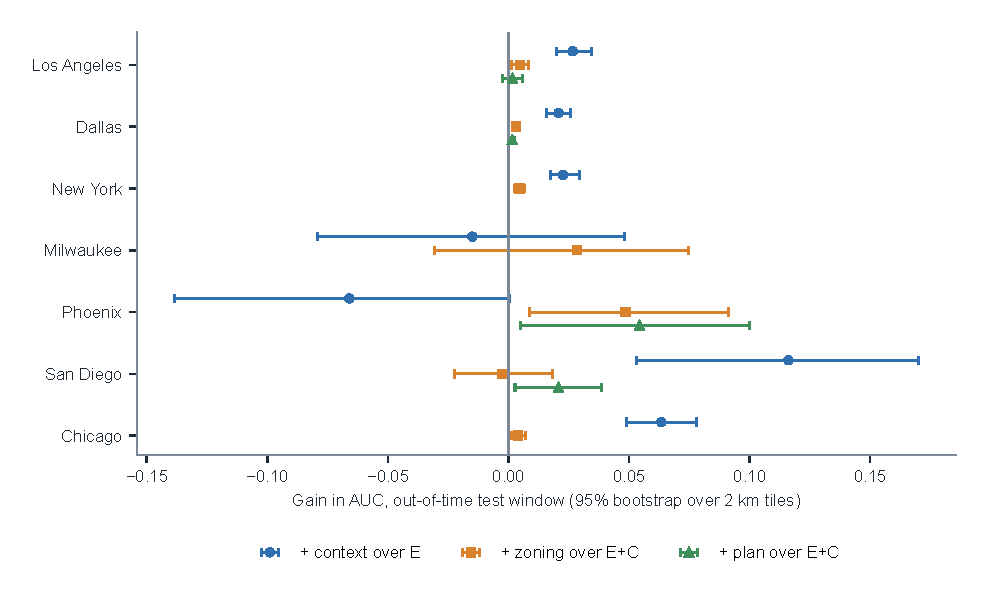
\includegraphics[width=0.8\linewidth]{Fig5}
\caption{Gain in out-of-time AUC from each block, with 95\% tile-bootstrap intervals}
\label{fig:gains}
\end{figure}

\begin{table}[t]
\centering
\scriptsize
\setlength{\tabcolsep}{4pt}
\caption{What developed lots became: share named correctly, as one of 16 classes / one of nine groups.}
\label{tab:dest}
\begin{tabular}{lrllll}
\toprule
City & Developed & No change & Zoning class & Plan class & Model (blocks) \\
\midrule
Los Angeles & 1{,}877 & 57\% / 79\% & 70\% / 87\% & 70\% / 87\% & 75\% / 89\% (E+C+Z+P) \\
Dallas & 3{,}886 & 37\% / 40\% & 61\% / 65\% & 80\% / 90\% & 86\% / 96\% (E+C+Z+P) \\
New York & 4{,}002 & 24\% / 37\% & 49\% / 65\% & -- & 54\% / 70\% (E+Z) \\
Milwaukee & 78 & 18\% / 18\% & 37\% / 77\% & -- & 63\% / 76\% (E+Z) \\
Phoenix & 1{,}835 & 0\% / 35\% & 64\% / 74\% & 47\% / 62\% & 75\% / 81\% (E+C+Z+P) \\
San Diego & 202 & 0\% / 52\% & 14\% / 74\% & 27\% / 70\% & 64\% / 75\% (E+C+Z+P) \\
\bottomrule
\end{tabular}
\par\smallskip
\begin{minipage}{0.95\linewidth}\footnotesize In Phoenix and San Diego development is a change of class (to another group, or to more homes), so ``no change'' is never right at class level there. Models are cross-fitted over 2 km tiles among the developed lots. Chicago's permits do not record the new use.\end{minipage}
\end{table}

\subsection{Housing projections}\label{sec:r-homes}

Projections and observations differ in kind: build-out is an end state, while the observed count is the gross number
of homes added in a two- or four-year window (Table~\ref{tab:homes}).
\begin{itemize}
\item \textbf{Ranking districts.} A five-year trend ranks districts better than build-out and likelihood $\times$
build-out in all four cities: Spearman 0.51 to 0.81, against $-$0.37 to 0.55.
Likelihood $\times$ empirical yield (below) reaches $-$0.28 to 0.83, as well as the trend or better
in three of four.
\item \textbf{Build-out.} A proxy of zoning and plan build-out (each lot at the density that lots of its zoned or
planned class reach today, not legal capacity) exceeds the homes added in the window 76- to 193-fold.
\item \textbf{Totals.} Likelihood weighting brings totals to 0.80--2.60 times the observed. Using the homes
that developing lots of the same class and size added in the training window instead of build-out gives
0.12--0.45: it ranks districts well but underestimates how many homes are built.
\item \textbf{Manhattan rezonings} (Table~\ref{tab:replay}, Figure~\ref{fig:replay}). Capacity projected
8{,}423 homes on development sites, or 5{,}207 pro-rated to 2025; 561 were built.
Probability $\times$ capacity gave 607, but the close total comes from errors that cancel: 0.84 and
0.87 times the observed in East Harlem and Inwood, and 44 times in SoHo/NoHo, where
3 homes were built. Soft sites redeveloped in the training years added 38\%--102\% of their capacity
homes on average; scaling by that share gives 352 in total and a larger summed error across the three
(471 homes, against 212), so the empirical yield did not improve these projections. The observed
count lies within the 95\% range of probability $\times$ capacity in two of three rezonings; the ranges are conditional
on the model's probabilities and omit model error.
\end{itemize}

\begin{table}[t]
\centering
\scriptsize
\setlength{\tabcolsep}{3pt}
\caption{Homes added in the test window: projection over observed total (Spearman correlation across districts).}
\label{tab:homes}
\begin{tabular}{lrllllll}
\toprule
City & Observed & Zoning build-out & Plan build-out & Likely $\times$ zoning & Likely $\times$ plan & Likely $\times$ yield & Five-year trend \\
\midrule
Los Angeles & 22{,}853 & 193$\times$ (0.10) & 189$\times$ (0.24) & 0.80$\times$ (0.51) & 0.81$\times$ (0.54) & 0.33$\times$ (0.79) & 0.59$\times$ (0.70) \\
Dallas & 10{,}926 & 141$\times$ (0.00) & 127$\times$ (0.34) & 2.60$\times$ ($-$0.05) & 1.59$\times$ (0.33) & 0.45$\times$ (0.73) & 1.25$\times$ (0.72) \\
New York & 116{,}776 & 76$\times$ (0.34) & -- & 0.96$\times$ (0.55) & -- & 0.37$\times$ (0.83) & 0.47$\times$ (0.81) \\
Milwaukee & 3{,}798 & 115$\times$ ($-$0.23) & -- & 0.97$\times$ ($-$0.37) & -- & 0.12$\times$ ($-$0.28) & 0.32$\times$ (0.51) \\
\bottomrule
\end{tabular}
\par\smallskip
\begin{minipage}{0.95\linewidth}\footnotesize Observed: gross homes added in the window. Build-out (a proxy, not legal capacity): every lot at the homes per hectare that the 90th percentile of lots of its zoned (or planned) class reach in the city today. Likely: the build-out increment times the out-of-time probability of development (blocks E+C+Z+P where available). Yield: the probability times the mean homes added by developing lots of the same class and lot size in the training window. Trend: homes completed in the five years before the window, scaled to its length.\end{minipage}
\end{table}

\begin{table}[t]
\centering
\footnotesize
\setlength{\tabcolsep}{3pt}
\caption{Three Manhattan rezonings: homes on development sites by 2025, observed and projected.}
\label{tab:replay}
\begin{tabular}{lrrrrll}
\toprule
Rezoning (adopted) & Sites & Built & Capacity & Pro-rated & Prob.\ $\times$ capacity (95\%) & Prob.\ $\times$ yield (95\%) \\
\midrule
East Harlem (2017) & 127 & 288 & 4{,}117 & 3{,}294 & 241 (82--497) & 91 (0--444) \\
Inwood (2018) & 47 & 270 & 2{,}859 & 1{,}334 & 234 (0--677) & 127 (0--1{,}033) \\
SoHo/NoHo (2021) & 77 & 3 & 1{,}447 & 579 & 132 (8--296) & 134 (0--801) \\
\textit{All three} &  & 561 & 8{,}423 & 5{,}207 & 607 & 352 \\
\textit{Sum of absolute errors} &  &  & 7{,}862 & 4{,}646 & 212 & 471 \\
\bottomrule
\end{tabular}
\par\smallskip
\begin{minipage}{0.95\linewidth}\footnotesize Capacity is full build-out by the review's build year; pro-rated scales it linearly to 2025. The probability comes from a redevelopment model trained only on outcomes known by the adoption year; yield is the mean share of capacity homes that soft sites redeveloped in those training years added. Ranges are conditional on the probabilities (Supplement S5).\end{minipage}
\end{table}

\begin{figure}[t]
\centering
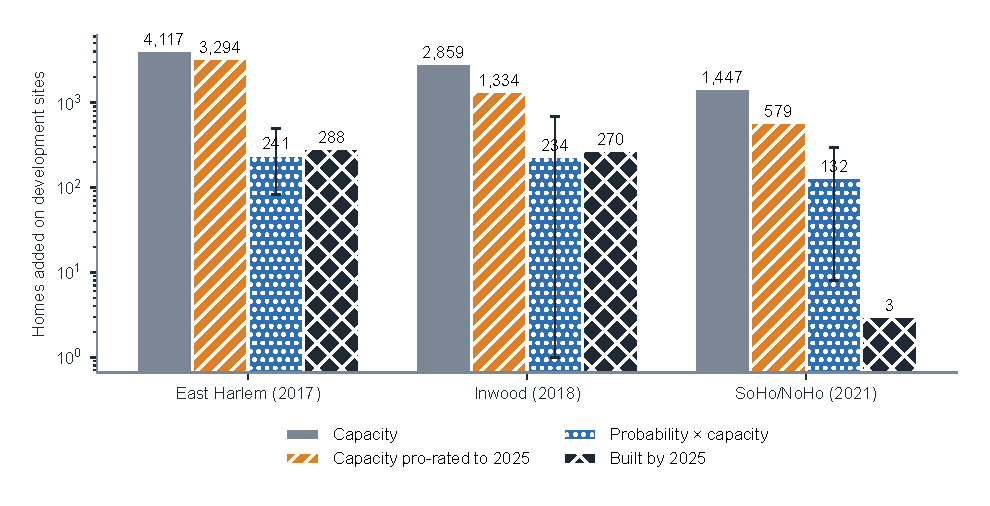
\includegraphics[width=0.8\linewidth]{Fig6}
\caption{Homes on development sites after three Manhattan rezonings: capacity, pro-rated capacity,
probability $\times$ capacity (with its 95\% range, conditional on the probabilities) and built by 2025 (log scale)}
\label{fig:replay}
\end{figure}

\subsection{Optimizer and plausibility}\label{sec:r-opt}

\paragraph{Optimality} (algorithmic verification). In 20 small areas (one tax block each) every plan with up
to two changes was enumerated, and 15 had a plan better than no change. First-order search found the optimum
in 14 of 15 of these, and with exact re-scoring in all 15 (median 0.51 s). At district
scale no method guarantees an optimum, so methods are compared with the best plan any of them found
(Table~\ref{tab:opt}): exact greedy search found it in all 12 districts but took a median 36.15 s;
first-order search with re-scoring reached a median 95.7\% of it in 1.88 s, the speed used in
the Studio.

\paragraph{Trade-off front.} On 10 tax blocks with 24{,}576--327{,}680 possible plans each, the NSGA-III
explorer's front covered a median 100.0\% (minimum 98.6\%) of the hypervolume of the exhaustive
front, against 96.4\% for random search with as many evaluations; on 10 smaller blocks scored
exactly, it recovered the exact front. The test exposed terms missing from the first-order model, since added
(Online Resource 1, Sect.~S6).

\paragraph{Plausibility} (Table~\ref{tab:realism}). Plans were recommended on the 2020 snapshot and compared with 2025,
with the same number of recommended parcels in each setting and one objective.
\begin{itemize}
\item \textbf{Precedent.} Without realism layers, 17\% of recommended changes had no precedent.
\item \textbf{Redevelopment.} Recommended parcels were redeveloped by 2025 at 11\% without realism layers,
15\% with the precedent filter and 21\% with the likelihood layer, against 1.2\% of all lots
and 5.0\% of the likeliest fifth.
\item \textbf{Redevelopment is not implementation.} None of the recommended parcels became the recommended use.
\item \textbf{The cost.} The objective fell by 3\% with the precedent filter and 48\% with the
likelihood layer: the filter removes implausible conversions at little cost, while restricting candidates to likely
sites trades much of the objective for plausibility.
\end{itemize}

\begin{table}[t]
\centering
\small
\setlength{\tabcolsep}{4pt}
\caption{Optimizer at district scale (12 Manhattan districts, up to ten changes): share of the best plan any tested method found (not a proven optimum).}
\label{tab:opt}
\begin{tabular}{lrrr}
\toprule
Search & Median share of best & Districts best & Median seconds \\
\midrule
surrogate top moves & 91.0\% & 0 & 0.02 \\
first order & 94.1\% & 0 & 0.25 \\
first order plus exact polish & 95.7\% & 1 & 1.88 \\
greedy exact & 100.0\% & 12 & 36.15 \\
simulated annealing & 93.6\% & 0 & 10.65 \\
random restarts 50 & 65.5\% & 0 & 1.31 \\
\bottomrule
\end{tabular}
\end{table}

\begin{table}[t]
\centering
\scriptsize
\setlength{\tabcolsep}{4pt}
\caption{Realism layers at equal counts: plans recommended on the 2020 snapshot of every Manhattan district, and what happened by 2025.}
\label{tab:realism}
\begin{tabular}{lrrrrrr}
\toprule
Optimizer setting & Parcels & No precedent & Redeveloped & Eligible redev. & Into rec.\ use & Objective \\
\midrule
no realism layer & 116 & 16.4\% & 11.2\% & 1.5\% & 0.0\% & 83.7 \\
precedent filter (default) & 117 & 0.0\% & 15.4\% & 1.5\% & 0.0\% & 81.3 \\
precedent filter + likelihood layer & 118 & 0.0\% & 21.2\% & 5.0\% & 0.0\% & 43.4 \\
\bottomrule
\end{tabular}
\par\smallskip
\begin{minipage}{0.95\linewidth}\footnotesize In each district every setting recommends the smallest number any setting recommended there. Eligible redev.: share of the setting's eligible parcels redeveloped (the rate of a random choice). Objective: the sum over districts of the overall score minus the conversion penalty. At the full budget the settings recommended 539, 543, 118 parcels.\end{minipage}
\end{table}

\subsection{Decision rules (illustrative)}\label{sec:r-dec}

The decision module has no observed counterpart: its outputs follow from assumed utilities, one seat per agent and the
generated candidates. In the simulated scenario for 12 Manhattan districts:
\begin{itemize}
\item the nine rules never all agree, and a Condorcet winner exists in seven;
\item the residents' referendum picks the council's plan in one district, and the council's winner
is never the Nash bargaining solution;
\item one insincere ballot could change the Schulze result in eight districts;
\item the winner survives a median 68\% of joint perturbations of coefficients and seats, and 58\%
of redrawn agent weights;
\item the candidates matter: the nine rules pick a median of four distinct winners on the generated
ballot, three on the agents' ideal plans alone and two on random feasible plans;
\item with resident weights drawn independently for each block, the residents' winner is unchanged in a median
100\% of draws.
\end{itemize}
These describe the simulated scenario, not public opinion. They make explicit what a hearing leaves implicit: resident
and environmental interests are inputs to the decision, and a recommendation should be reported with its rule, its
candidates and how it changes under others.

\section{Discussion}\label{sec:discussion}

\paragraph{What a planner gets.} For any proposed change, PlanArena shows:
\begin{itemize}
\item its effects on 11 indicators, with ranges;
\item whether zoning and the plan allow it, and how likely it is;
\item what the optimizer would recommend instead;
\item how the choice depends on the decision rule.
\end{itemize}
Each output has a stated test and type of evidence (Table~\ref{tab:design}), and untested indicators are
labelled. For one system, this narrows the gap between claimed and demonstrated contributions of PSS and urban twins
\citep{vonk2005,azadi2025,kruse2026}.

\paragraph{Design guidance.}
\begin{enumerate}
\item \textbf{Use each layer for the question it answers.} Once existing conditions and context were known, zoning and
plans added little to ranking \emph{where} development happened in these windows. They helped name \emph{what} it
became and bound \emph{how much} a site can hold. This is consistent with rezoning following opportunity \citep{gabbe2018},
upzoning's varying short-run effects \citep{freemark2020,dong2024,greenaway2023} and partial plan implementation
\citep{laurian2004,berke2006}.
\item \textbf{Report a trend first, and likelihood-weighted projections beside capacity.} Capacity overstates
near-term housing by orders of magnitude. A trend ranked districts better than build-out-based projections in all four cities, and likelihood $\times$ yield as well as the trend in three of four. Close totals can hide large errors by area.
\item \textbf{Constrain optimization by plausibility and show the cost.} Realism layers change recommendations and
lower the objective; recommended sites that redevelop rarely become the recommended use.
\item \textbf{Report decisions with their rule.} No rule agreed with all the others in any district of the simulated scenario.
\end{enumerate}

\paragraph{Limitations.}
\begin{itemize}
\item \textbf{Impacts} are evaluated only in Manhattan and only given what was built; in the other nine cities they
are unvalidated estimates from national or regional coefficients.
\item \textbf{Indicators without skill or test.} Job change by block was tested and showed no skill; access, mix,
green cover and runoff after a change have no observed test.
\item \textbf{Calibration.} Redevelopment probabilities shift with the market cycle, so expected totals need checking
against recent rates.
\item \textbf{The cross-city test} uses short windows (one or two years) and city-specific outcome definitions, and
Dallas's undated layers may include post-decision information.
\item \textbf{Representation.} Zoning is reduced to use permissions and maximum floor-area ratios (no height, bulk,
parking or bonus rules), access to straight-line distance, and uncertainty to sensitivity ranges, which are not
prediction intervals.
\item \textbf{Distribution.} Indicators are averages over a scope. Who gains and who loses within it (by income,
tenure or race), displacement and the effects on future residents are not measured.
\item \textbf{Decisions.} The optimizer is heuristic, and the votes rest on assumed utilities and one seat per
interest, not on elicited preferences or representation.
\item \textbf{Not studied.} Usability with planners is not evaluated, and causal effects of zoning or plans are not
estimated.
\end{itemize}

\section{Conclusion}

Land-use and location decisions have multidimensional, spatially interacting and uncertain effects, yet they are
decided at hearings where those effects are summarised in a few indicators and residents do not vote. PlanArena, a
land-use optimizer, measures the effects of any parcel-level change on social, economic and environmental
indicators, with what is permitted, planned, likely and recommended, and turns stakeholder interests into votes. It runs on official data for ten large US cities
at interactive speed, and each component has a stated test, empirical where data allow. The tests also shape the
design:
\begin{itemize}
\item once existing conditions and context are known, regulatory layers mainly inform what development becomes and
how much it could hold;
\item a five-year trend ranked districts better than build-out projections, and likelihood-weighted totals were far
closer to what was built than capacity, partly through errors that cancel;
\item recommendations change when they must be plausible, at a measured cost, and the chosen plan changes with the
rule and the candidates.
\end{itemize}
Code, data manifest and results are released with the paper, so the system and its tests extend to other cities.

\section*{Statements and Declarations}

\paragraph{Competing interests.} The author has no relevant financial or non-financial interests to disclose.

\paragraph{Funding.} No funding was received for conducting this study.

\paragraph{Ethics approval and consent.} Not applicable. The study uses public administrative records; it involves no
human participants or animals. Owner, mailing and taxpayer fields in assessor records were never requested or read.

\paragraph{Data availability.} All inputs are public and are downloaded by script; a manifest records each input's
URL, retrieval date and SHA-256, and the result file behind every number, the figures and each city's ingestion report
are in the repository below. The datasets are cited in the text and listed in the references.

\paragraph{Code availability.} The code is released under the MIT licence at \url{https://anonymous.4open.science/r/planarena-cus} (anonymised for
review); \texttt{make reproduce} rebuilds the data and every result. The online Studio and game are at
\url{https://planarena-manhattan.onrender.com} and \url{https://planarena-manhattan.onrender.com/play}.

\paragraph{Author contributions.} Given on the title page.

\appendix
\section{Digitising plans published as PDF maps}\label{app:digitise}

Philadelphia2035's land-use recommendations exist only as ``Proposed Land Use'' maps in 17 district plans
covering 18 districts. Each lot is a filled vector shape. The maps are converted in six steps:
\begin{enumerate}
\item \textbf{Legend.} Swatch colours and labels are read.
\item \textbf{Colour matching.} Map colours are matched one to one to legend colours by CIELAB $\Delta E$ with a
Hungarian assignment, refusing pairs with $\Delta E > 45$.
\item \textbf{Visibility.} Only shapes the rendered page shows are kept, since maps are often clipped to the
district, and only the largest map frame on the spread.
\item \textbf{Registration.} A similarity transform is fitted. The rendered footprint is matched as an image to the
district's parcels and outline (FFT translation, Dice score), then refined by iterative closest point
\citep{reddy1996,besl1992,umeyama1991}.
\item \textbf{Classification.} Each parcel takes the category of the smallest shape containing its interior point.
\item \textbf{Checks.} A map is used only if the median parcel-to-shape distance is at most 3.0 m (10 ft), and its plan
agrees with existing use clearly more often than the same map shifted 91 m (300 ft).
\end{enumerate}
Results:
\begin{itemize}
\item \textbf{Coverage.} Maps from 15 of 17 plans passed, covering 16
districts and 83\% of parcels.
\item \textbf{Registration.} Median errors were 0.3--2.2 m (median 1.0 m).
\item \textbf{Shifted-map control.} The digitised plans agree with existing use on 60\%--90\%
of parcels, against 42\%--66\% for shifted maps.
\item \textbf{Independent reading.} Each parcel's category was also read from the colour of the rendered page around
its point, matched to the legend's rendered colours. On 451{,}691 parcels read both ways, the two readings agree
on 99.8\% (99.4\%--100.0\% by district). Both use the same registration, which the shifted-map
control checks. A random sample of 150 parcels, with page positions and map crops, is provided for a check
by eye against the PDFs.
\item \textbf{Failures.} The maps of South and West Park also draw neighbouring districts and failed registration.
\end{itemize}
Earlier work addresses scanned raster maps \citep{chiang2014,luft2021,milleville2022}; vector exports allow shapes to
be read directly.

\begin{thebibliography}{}
\setlength{\itemsep}{1pt}
\bibitem[{Abolhasani et~al.}(2026){Abolhasani, Eudave, Hersperger}]{abolhasani2026}
Abolhasani, S., Eudave, R. R., \& Hersperger, A. M. (2026). Toward policy-informed 3D urban land-use simulations by leveraging urban planning regulations: Case studies in Zurich and Copenhagen. {\itshape Land Use Policy}, {\itshape 170}, 108189. \url{https://doi.org/10.1016/j.landusepol.2026.108189}
\bibitem[{Abolhasani et~al.}(2022){Abolhasani, Taleai, Lakes}]{abolhasani2022}
Abolhasani, S., Taleai, M., \& Lakes, T. (2022). A collective decision-making framework for simulating urban land-use planning: An application of game theory with event-driven actors. {\itshape Computers, Environment and Urban Systems}, {\itshape 94}, 101795. \url{https://doi.org/10.1016/j.compenvurbsys.2022.101795}
\bibitem[{Arnstein}(1969){Arnstein}]{arnstein1969}
Arnstein, S. R. (1969). A Ladder Of Citizen Participation. {\itshape Journal of the American Institute of Planners}, {\itshape 35}(4), 216–224. \url{https://doi.org/10.1080/01944366908977225}
\bibitem[{Azadi et~al.}(2025){Azadi, Kasraian, Nourian, van Wesemael}]{azadi2025}
Azadi, S., Kasraian, D., Nourian, P., \& van Wesemael, P. (2025). What Have Urban Digital Twins Contributed to Urban Planning and Decision Making? From a Systematic Literature Review Toward a Socio-Technical Research and Development Agenda. {\itshape Smart Cities}, {\itshape 8}(1), 32. \url{https://doi.org/10.3390/smartcities8010032}
\bibitem[{Batty}(2018){Batty}]{batty2018}
Batty, M. (2018). Digital twins. {\itshape Environment and Planning B: Urban Analytics and City Science}, {\itshape 45}(5), 817–820. \url{https://doi.org/10.1177/2399808318796416}
\bibitem[{Batty}(2024){Batty}]{batty2024}
Batty, M. (2024). Digital twins in city planning. {\itshape Nature Computational Science}, {\itshape 4}(3), 192–199. \url{https://doi.org/10.1038/s43588-024-00606-7}
\bibitem[{Berke et~al.}(2006){Berke, Backhurst, Day, Ericksen, Laurian, Crawford}]{berke2006}
Berke, P., Backhurst, M., Day, M., Ericksen, N., Laurian, L., Crawford, J., \& Dixon, J. (2006). What Makes Plan Implementation Successful? An Evaluation of Local Plans and Implementation Practices in New Zealand. {\itshape Environment and Planning B: Planning and Design}, {\itshape 33}(4), 581–600. \url{https://doi.org/10.1068/b31166}
\bibitem[{Besl \& McKay}(1992){Besl, McKay}]{besl1992}
Besl, P. J., \& McKay, N. D. (1992). A method for registration of 3-D shapes. {\itshape IEEE Transactions on Pattern Analysis and Machine Intelligence}, {\itshape 14}(2), 239–256. \url{https://doi.org/10.1109/34.121791}
\bibitem[{Bexar Appraisal District}(2025){Bexar Appraisal District}]{data_bexar}
Bexar Appraisal District. (2025). {\itshape Parcels (December 2025); with City of San Antonio Future Land Use and zoning} [Data set]. Retrieved October 2026, from \url{https://gis.sara-tx.org/ags1/rest/services/FW_Bexar/BCAD_Parcels_PROD/FeatureServer/0}
\bibitem[{Black et~al.}(2023){Black, van Strien, Adde, Grêt-Regamey}]{black2023}
Black, B., van Strien, M. J., Adde, A., \& Grêt-Regamey, A. (2023). Re-considering the status quo: Improving calibration of land use change models through validation of transition potential predictions. {\itshape Environmental Modelling \& Software}, {\itshape 159}, 105574. \url{https://doi.org/10.1016/j.envsoft.2022.105574}
\bibitem[{Brandt et~al.}(2016){Brandt, Conitzer, Endriss, Lang, Procaccia}]{brandt2016}
Brandt, F., Conitzer, V., Endriss, U., Lang, J., \& Procaccia, A. D. (Eds.). (2016). {\itshape Handbook of Computational Social Choice.} Cambridge University Press. \url{https://doi.org/10.1017/CBO9781107446984}
\bibitem[{Brody \& Highfield}(2005){Brody, Highfield}]{brody2005}
Brody, S. D., \& Highfield, W. E. (2005). Does Planning Work?: Testing the Implementation of Local Environmental Planning in Florida. {\itshape Journal of the American Planning Association}, {\itshape 71}(2), 159–175. \url{https://doi.org/10.1080/01944360508976690}
\bibitem[{Carruthers \& Wei}(2024){Carruthers, Wei}]{carruthers2024}
Carruthers, J. I., \& Wei, H. (2024). What drives urban redevelopment activity? Evidence from machine learning and econometric analysis in three American cities. {\itshape Journal of Geographical Systems}, {\itshape 26}(4), 565–599. \url{https://doi.org/10.1007/s10109-024-00451-2}
\bibitem[{Charles}(2013){Charles}]{charles2013}
Charles, S. L. (2013). Understanding the Determinants of Single-family Residential Redevelopment in the Inner-ring Suburbs of Chicago. {\itshape Urban Studies}, {\itshape 50}(8), 1505–1522. \url{https://doi.org/10.1177/0042098012465908}
\bibitem[{Chiang et~al.}(2014){Chiang, Leyk, Knoblock}]{chiang2014}
Chiang, Y.-Y., Leyk, S., \& Knoblock, C. A. (2014). A Survey of Digital Map Processing Techniques. {\itshape ACM Computing Surveys}, {\itshape 47}(1), 1–44. \url{https://doi.org/10.1145/2557423}
\bibitem[{Chicago Metropolitan Agency for Planning}(n.d.){Chicago Metropolitan Agency for Planning}]{data_cmap}
Chicago Metropolitan Agency for Planning. (n.d.). {\itshape Land Use Inventory 2023; with Cook County parcels 2025 and Cook County Assessor records} [Data set]. Retrieved October 2026, from \url{https://www.cmap.illinois.gov/data/land-use/inventory}
\bibitem[{Church \& ReVelle}(1974){Church, ReVelle}]{church1974}
Church, R., \& ReVelle, C. (1974). The maximal covering location problem. {\itshape Papers of the Regional Science Association}, {\itshape 32}(1), 101–118. \url{https://doi.org/10.1007/bf01942293}
\bibitem[{City of Dallas}(n.d.){City of Dallas}]{data_dallas}
City of Dallas. (n.d.). {\itshape Existing Land Use (2026), forwardDallas! 2.0 placetypes (2024) and base zoning; with Dallas Central Appraisal District 2026 certified data} [Data set]. Retrieved October 2026, from \url{https://services2.arcgis.com/rwnOSbfKSwyTBcwN/arcgis/rest/services/Existing_Land_Use_Layer_2025/FeatureServer/5}
\bibitem[{City of Houston}(n.d.){City of Houston}]{data_houston}
City of Houston. (n.d.). {\itshape Land Use (Grouped), from Harris Central Appraisal District records} [Data set]. Retrieved October 2026, from \url{https://mycity2.houstontx.gov/gisweb02/rest/services/HoustonMap/Landuse/MapServer/0}
\bibitem[{City of Milwaukee}(n.d.){City of Milwaukee}]{data_mprop}
City of Milwaukee. (n.d.). {\itshape Master Property File (MPROP), assessment years 2015 to 2026, and parcel polygons} [Data set]. Retrieved October 2026, from \url{https://data.milwaukee.gov/dataset/mprop}
\bibitem[{City of Philadelphia}(n.d.){City of Philadelphia}]{data_opa}
City of Philadelphia. (n.d.). {\itshape Philadelphia Properties and Assessment History; with Philadelphia Water Department parcels (OpenDataPhilly)} [Data set]. Retrieved October 2026, from \url{https://opendataphilly.org/datasets/philadelphia-properties-and-assessment-history/}
\bibitem[{Clarke et~al.}(1997){Clarke, Hoppen, Gaydos}]{clarke1997}
Clarke, K. C., Hoppen, S., \& Gaydos, L. (1997). A Self-Modifying Cellular Automaton Model of Historical Urbanization in the San Francisco Bay Area. {\itshape Environment and Planning B: Planning and Design}, {\itshape 24}(2), 247–261. \url{https://doi.org/10.1068/b240247}
\bibitem[{Deb \& Jain}(2014){Deb, Jain}]{deb2014}
Deb, K., \& Jain, H. (2014). An Evolutionary Many-Objective Optimization Algorithm Using Reference-Point-Based Nondominated Sorting Approach, Part I: Solving Problems With Box Constraints. {\itshape IEEE Transactions on Evolutionary Computation}, {\itshape 18}(4), 577–601. \url{https://doi.org/10.1109/tevc.2013.2281535}
\bibitem[{Domingo et~al.}(2021){Domingo, Palka, Hersperger}]{domingo2021}
Domingo, D., Palka, G., \& Hersperger, A. M. (2021). Effect of zoning plans on urban land-use change: A multi-scenario simulation for supporting sustainable urban growth. {\itshape Sustainable Cities and Society}, {\itshape 69}, 102833. \url{https://doi.org/10.1016/j.scs.2021.102833}
\bibitem[{Dong}(2024){Dong}]{dong2024}
Dong, H. (2024). Exploring the Impacts of Zoning and Upzoning on Housing Development: A Quasi-experimental Analysis at the Parcel Level. {\itshape Journal of Planning Education and Research}, {\itshape 44}(1), 403–415. \url{https://doi.org/10.1177/0739456x21990728}
\bibitem[{Dye \& McMillen}(2007){Dye, McMillen}]{dye2007}
Dye, R. F., \& McMillen, D. P. (2007). Teardowns and land values in the Chicago metropolitan area. {\itshape Journal of Urban Economics}, {\itshape 61}(1), 45–63. \url{https://doi.org/10.1016/j.jue.2006.06.003}
\bibitem[{Einstein et~al.}(2019){Einstein, Palmer, Glick}]{einstein2019}
Einstein, K. L., Palmer, M., \& Glick, D. M. (2019). Who Participates in Local Government? Evidence from Meeting Minutes. {\itshape Perspectives on Politics}, {\itshape 17}(1), 28–46. \url{https://doi.org/10.1017/s153759271800213x}
\bibitem[{Feng et~al.}(2024){Feng, Hou, Jiang, Shi}]{feng2024}
Feng, H., Hou, J., Jiang, J., \& Shi, L. (2024). Land Use Optimization from the Perspective of Multiple Stakeholder Groups: A Case Study in Yongsheng County, Yunnan Province, China. {\itshape Land}, {\itshape 13}(10), 1593. \url{https://doi.org/10.3390/land13101593}
\bibitem[{Ferré-Bigorra et~al.}(2022){Ferré-Bigorra, Casals, Gangolells}]{ferrebigorra2022}
Ferré-Bigorra, J., Casals, M., \& Gangolells, M. (2022). The adoption of urban digital twins. {\itshape Cities}, {\itshape 131}, 103905. \url{https://doi.org/10.1016/j.cities.2022.103905}
\bibitem[{Freemark}(2020){Freemark}]{freemark2020}
Freemark, Y. (2020). Upzoning Chicago: Impacts of a Zoning Reform on Property Values and Housing Construction. {\itshape Urban Affairs Review}, {\itshape 56}(3), 758–789. \url{https://doi.org/10.1177/1078087418824672}
\bibitem[{Fung}(2006){Fung}]{fung2006}
Fung, A. (2006). Varieties of Participation in Complex Governance. {\itshape Public Administration Review}, {\itshape 66}(s1), 66–75. \url{https://doi.org/10.1111/j.1540-6210.2006.00667.x}
\bibitem[{Gabbe}(2018){Gabbe}]{gabbe2018}
Gabbe, C. J. (2018). Why Are Regulations Changed? A Parcel Analysis of Upzoning in Los Angeles. {\itshape Journal of Planning Education and Research}, {\itshape 38}(3), 289–300. \url{https://doi.org/10.1177/0739456x17696034}
\bibitem[{Geertman \& Stillwell}(2020){Geertman, Stillwell}]{geertman2020}
Geertman, S., \& Stillwell, J. (2020). Planning support science: Developments and challenges. {\itshape Environment and Planning B: Urban Analytics and City Science}, {\itshape 47}(8), 1326–1342. \url{https://doi.org/10.1177/2399808320936277}
\bibitem[{Greenaway-McGrevy \& Phillips}(2023){Greenaway-McGrevy, Phillips}]{greenaway2023}
Greenaway-McGrevy, R., \& Phillips, P. C. B. (2023). The impact of upzoning on housing construction in Auckland. {\itshape Journal of Urban Economics}, {\itshape 136}, 103555. \url{https://doi.org/10.1016/j.jue.2023.103555}
\bibitem[{Hashemi et~al.}(2026){Hashemi, Taleai, Abolhasani}]{hashemi2026}
Hashemi, V., Taleai, M., \& Abolhasani, S. (2026). Negotiation‐Aware Optimization Approach for Multi‐Stakeholder Agricultural Land Reallocation: A Case Study in Iran. {\itshape Transactions in GIS}, {\itshape 30}(5). \url{https://doi.org/10.1111/tgis.70331}
\bibitem[{Hersperger et~al.}(2018){Hersperger, Oliveira, Pagliarin, Palka, Verburg, Bolliger}]{hersperger2018}
Hersperger, A. M., Oliveira, E., Pagliarin, S., Palka, G., Verburg, P., Bolliger, J., \& Grădinaru, S. (2018). Urban land-use change: The role of strategic spatial planning. {\itshape Global Environmental Change}, {\itshape 51}, 32–42. \url{https://doi.org/10.1016/j.gloenvcha.2018.05.001}
\bibitem[{Innes \& Booher}(2004){Innes, Booher}]{innes2004}
Innes, J. E., \& Booher, D. E. (2004). Reframing public participation: strategies for the 21st century. {\itshape Planning Theory \& Practice}, {\itshape 5}(4), 419–436. \url{https://doi.org/10.1080/1464935042000293170}
\bibitem[{Klosterman}(1999){Klosterman}]{klosterman1999}
Klosterman, R. E. (1999). The What If? Collaborative Planning Support System. {\itshape Environment and Planning B: Planning and Design}, {\itshape 26}(3), 393–408. \url{https://doi.org/10.1068/b260393}
\bibitem[{Kruse et~al.}(2026){Kruse, Nielsen, de Neergaard}]{kruse2026}
Kruse, E. N., Nielsen, T. T., \& de Neergaard, M. (2026). From epistemic promises to real world practices: the ongoing becoming of 3D models and urban digital twins in municipal planning. {\itshape Computational Urban Science}, {\itshape 6}(1). \url{https://doi.org/10.1007/s43762-026-00299-w}
\bibitem[{Kunsch}(1989){Kunsch}]{kunsch1989}
Kunsch, H. R. (1989). The Jackknife and the Bootstrap for General Stationary Observations. {\itshape The Annals of Statistics}, {\itshape 17}(3), 1217–1241. \url{https://doi.org/10.1214/aos/1176347265}
\bibitem[{Landis \& Zhang}(1998){Landis, Zhang}]{landis1998}
Landis, J., \& Zhang, M. (1998). The Second Generation of the California Urban Futures Model. Part 1: Model Logic and Theory. {\itshape Environment and Planning B: Planning and Design}, {\itshape 25}(5), 657–666. \url{https://doi.org/10.1068/b250657}
\bibitem[{Laurian et~al.}(2004){Laurian, Day, Berke, Ericksen, Backhurst, Crawford}]{laurian2004}
Laurian, L., Day, M., Berke, P., Ericksen, N., Backhurst, M., Crawford, J., \& Dixon, J. (2004). Evaluating Plan Implementation: A Conformance-Based Methodology. {\itshape Journal of the American Planning Association}, {\itshape 70}(4), 471–480. \url{https://doi.org/10.1080/01944360408976395}
\bibitem[{Lehtola et~al.}(2022){Lehtola, Koeva, Elberink, Raposo, Virtanen, Vahdatikhaki}]{lehtola2022}
Lehtola, V. V., Koeva, M., Elberink, S. O., Raposo, P., Virtanen, J.-P., Vahdatikhaki, F., \& Borsci, S. (2022). Digital twin of a city: Review of technology serving city needs. {\itshape International Journal of Applied Earth Observation and Geoinformation}, {\itshape 114}, 102915. \url{https://doi.org/10.1016/j.jag.2022.102915}
\bibitem[{Lei et~al.}(2023){Lei, Janssen, Stoter, Biljecki}]{lei2023}
Lei, B., Janssen, P., Stoter, J., \& Biljecki, F. (2023). Challenges of urban digital twins: A systematic review and a Delphi expert survey. {\itshape Automation in Construction}, {\itshape 147}, 104716. \url{https://doi.org/10.1016/j.autcon.2022.104716}
\bibitem[{Lin et~al.}(2025){Lin, Liu, Yuan, Wang, Li, Zhou}]{lin2025}
Lin, C., Liu, Y., Yuan, Z., Wang, H., Li, G., Zhou, Z., Wang, H., \& An, X. (2025). Harmonizing stakeholder interests in urban renewal: A novel planning approach using explainable machine learning and spatial optimization. {\itshape Land Use Policy}, {\itshape 155}, 107588. \url{https://doi.org/10.1016/j.landusepol.2025.107588}
\bibitem[{Loh}(2011){Loh}]{loh2011}
Loh, C. G. (2011). Assessing and Interpreting Non-conformance in Land-use Planning Implementation. {\itshape Planning Practice \& Research}, {\itshape 26}(3), 271–287. \url{https://doi.org/10.1080/02697459.2011.580111}
\bibitem[{Luft \& Schiewe}(2021){Luft, Schiewe}]{luft2021}
Luft, J., \& Schiewe, J. (2021). Automatic content‐based georeferencing of historical topographic maps. {\itshape Transactions in GIS}, {\itshape 25}(6), 2888–2906. \url{https://doi.org/10.1111/tgis.12794}
\bibitem[{Luo et~al.}(2025){Luo, Liu, Kong, Shen, Wu, Da Xu}]{luo2025}
Luo, J., Liu, P., Kong, X., Shen, J., Wu, Q., \& Da Xu. (2025). Urban digital twins for citizen-centric planning: A systematic review of built environment perception and public participation. {\itshape International Journal of Applied Earth Observation and Geoinformation}, {\itshape 143}, 104746. \url{https://doi.org/10.1016/j.jag.2025.104746}
\bibitem[{Malczewski}(2006){Malczewski}]{malczewski2006}
Malczewski, J. (2006). GIS‐based multicriteria decision analysis: a survey of the literature. {\itshape International Journal of Geographical Information Science}, {\itshape 20}(7), 703–726. \url{https://doi.org/10.1080/13658810600661508}
\bibitem[{Maricopa County Assessor}(n.d.){Maricopa County Assessor}]{data_maricopa}
Maricopa County Assessor. (n.d.). {\itshape Parcels (property use codes); with MAG Existing Land Use 2026 and City of Phoenix General Plan and zoning} [Data set]. Retrieved October 2026, from \url{https://maps.phoenix.gov/pub/rest/services/Public/COUNTY_PARCELS/MapServer/3}
\bibitem[{Meyer \& Pebesma}(2021){Meyer, Pebesma}]{meyer2021}
Meyer, H., \& Pebesma, E. (2021). Predicting into unknown space? Estimating the area of applicability of spatial prediction models. {\itshape Methods in Ecology and Evolution}, {\itshape 12}(9), 1620–1633. \url{https://doi.org/10.1111/2041-210x.13650}
\bibitem[{Milleville et~al.}(2022){Milleville, Verstockt, Van de Weghe}]{milleville2022}
Milleville, K., Verstockt, S., \& Van de Weghe, N. (2022). Automatic Georeferencing of Topographic Raster Maps. {\itshape ISPRS International Journal of Geo-Information}, {\itshape 11}(7), 387. \url{https://doi.org/10.3390/ijgi11070387}
\bibitem[{Nash}(1950){Nash}]{nash1950}
Nash, J. F. (1950). The Bargaining Problem. {\itshape Econometrica}, {\itshape 18}(2), 155. \url{https://doi.org/10.2307/1907266}
\bibitem[{New York City Department of Buildings}(2016){New York City Department of Buildings}]{data_ll84_2015}
New York City Department of Buildings. (2016). {\itshape Energy and Water Data Disclosure for Local Law 84 2016 (Data for Calendar Year 2015)} [Data set]. NYC Open Data. Retrieved October 2026, from \url{https://data.cityofnewyork.us/d/77q4-nkfh}
\bibitem[{New York City Department of Buildings}(2023){New York City Department of Buildings}]{data_ll84_2023}
New York City Department of Buildings. (2023). {\itshape NYC Building Energy and Water Data Disclosure for Local Law 84 2023 to Present (Data for Calendar Year 2022-Present)} [Data set]. NYC Open Data. Retrieved October 2026, from \url{https://data.cityofnewyork.us/d/5zyy-y8am}
\bibitem[{New York City Department of City Planning}(2017){New York City Department of City Planning}]{data_feis_eh}
New York City Department of City Planning. (2017). {\itshape East Harlem Rezoning Final Environmental Impact Statement, Appendix A} [Data set]. Retrieved October 2026, from \url{https://www.nyc.gov/assets/planning/download/pdf/applicants/env-review/east-harlem/appenda_feis.pdf}
\bibitem[{New York City Department of City Planning}(2021){New York City Department of City Planning}]{data_feis_sn}
New York City Department of City Planning. (2021). {\itshape SoHo/NoHo Neighborhood Plan Final Environmental Impact Statement, Appendix A} [Data set]. Retrieved October 2026, from \url{https://www.nyc.gov/assets/planning/download/pdf/applicants/env-review/soho-noho/appenda-feis.pdf}
\bibitem[{New York City Department of City Planning}(2025){New York City Department of City Planning}]{data_mappluto}
New York City Department of City Planning. (2025). {\itshape MapPLUTO, releases 15v1 to 25v3.1} [Data set]. Retrieved October 2026, from \url{https://www.nyc.gov/content/planning/pages/resources/datasets/mappluto-pluto-change}
\bibitem[{Parker et~al.}(2003){Parker, Manson, Janssen, Hoffmann, Deadman}]{parker2003}
Parker, D. C., Manson, S. M., Janssen, M. A., Hoffmann, M. J., \& Deadman, P. (2003). Multi-Agent Systems for the Simulation of Land-Use and Land-Cover Change: A Review. {\itshape Annals of the Association of American Geographers}, {\itshape 93}(2), 314–337. \url{https://doi.org/10.1111/1467-8306.9302004}
\bibitem[{Pelzer}(2017){Pelzer}]{pelzer2017}
Pelzer, P. (2017). Usefulness of planning support systems: A conceptual framework and an empirical illustration. {\itshape Transportation Research Part A: Policy and Practice}, {\itshape 104}, 84–95. \url{https://doi.org/10.1016/j.tra.2016.06.019}
\bibitem[{Philadelphia City Planning Commission}(n.d.){Philadelphia City Planning Commission}]{data_phila2035}
Philadelphia City Planning Commission. (n.d.). {\itshape Philadelphia2035 district plans} [Data set]. Retrieved October 2026, from \url{https://www.phila2035.org/plan}
\bibitem[{Ploton et~al.}(2020){Ploton, Mortier, Réjou-Méchain, Barbier, Picard, Rossi}]{ploton2020}
Ploton, P., Mortier, F., Réjou-Méchain, M., Barbier, N., Picard, N., Rossi, V., Dormann, C., Cornu, G., Viennois, G., Bayol, N., Lyapustin, A., Gourlet-Fleury, S., \& Pélissier, R. (2020). Spatial validation reveals poor predictive performance of large-scale ecological mapping models. {\itshape Nature Communications}, {\itshape 11}(1). \url{https://doi.org/10.1038/s41467-020-18321-y}
\bibitem[{Pontius et~al.}(2008){Pontius, Boersma, Castella, Clarke, de Nijs, Dietzel}]{pontius2008}
Pontius, R. G., Boersma, W., Castella, J.-C., Clarke, K., de Nijs, T., Dietzel, C., Duan, Z., Fotsing, E., Goldstein, N., Kok, K., Koomen, E., Lippitt, C. D., McConnell, W., Mohd Sood, A., Pijanowski, B., Pithadia, S., Sweeney, S., Trung, T. N., Veldkamp, A. T., \& Verburg, P. H. (2008). Comparing the input, output, and validation maps for several models of land change. {\itshape The Annals of Regional Science}, {\itshape 42}(1), 11–37. \url{https://doi.org/10.1007/s00168-007-0138-2}
\bibitem[{Pontius \& Millones}(2011){Pontius, Millones}]{pontius2011}
Pontius, R. G., \& Millones, M. (2011). Death to Kappa: birth of quantity disagreement and allocation disagreement for accuracy assessment. {\itshape International Journal of Remote Sensing}, {\itshape 32}(15), 4407–4429. \url{https://doi.org/10.1080/01431161.2011.552923}
\bibitem[{Rahman \& Szabó}(2021){Rahman, Szabó}]{rahman2021}
Rahman, M. M., \& Szabó, G. (2021). Multi-objective urban land use optimization using spatial data: A systematic review. {\itshape Sustainable Cities and Society}, {\itshape 74}, 103214. \url{https://doi.org/10.1016/j.scs.2021.103214}
\bibitem[{Reddy \& Chatterji}(1996){Reddy, Chatterji}]{reddy1996}
Reddy, B. S., \& Chatterji, B. N. (1996). An FFT-based technique for translation, rotation, and scale-invariant image registration. {\itshape IEEE Transactions on Image Processing}, {\itshape 5}(8), 1266–1271. \url{https://doi.org/10.1109/83.506761}
\bibitem[{ReVelle \& Eiselt}(2005){ReVelle, Eiselt}]{revelle2005}
ReVelle, C. S., \& Eiselt, H. A. (2005). Location analysis: A synthesis and survey. {\itshape European Journal of Operational Research}, {\itshape 165}(1), 1–19. \url{https://doi.org/10.1016/j.ejor.2003.11.032}
\bibitem[{Rittel \& Webber}(1973){Rittel, Webber}]{rittel1973}
Rittel, H. W. J., \& Webber, M. M. (1973). Dilemmas in a general theory of planning. {\itshape Policy Sciences}, {\itshape 4}(2), 155–169. \url{https://doi.org/10.1007/bf01405730}
\bibitem[{Roberts et~al.}(2017){Roberts, Bahn, Ciuti, Boyce, Elith, Guillera‐Arroita}]{roberts2017}
Roberts, D. R., Bahn, V., Ciuti, S., Boyce, M. S., Elith, J., Guillera‐Arroita, G., Hauenstein, S., Lahoz‐Monfort, J. J., Schröder, B., Thuiller, W., Warton, D. I., Wintle, B. A., Hartig, F., \& Dormann, C. F. (2017). Cross‐validation strategies for data with temporal, spatial, hierarchical, or phylogenetic structure. {\itshape Ecography}, {\itshape 40}(8), 913–929. \url{https://doi.org/10.1111/ecog.02881}
\bibitem[{Rosenthal \& Helsley}(1994){Rosenthal, Helsley}]{rosenthal1994}
Rosenthal, S. S., \& Helsley, R. W. (1994). Redevelopment and the Urban Land Price Gradient. {\itshape Journal of Urban Economics}, {\itshape 35}(2), 182–200. \url{https://doi.org/10.1006/juec.1994.1012}
\bibitem[{Saltelli et~al.}(2019){Saltelli, Aleksankina, Becker, Fennell, Ferretti, Holst}]{saltelli2019}
Saltelli, A., Aleksankina, K., Becker, W., Fennell, P., Ferretti, F., Holst, N., Li, S., \& Wu, Q. (2019). Why so many published sensitivity analyses are false: A systematic review of sensitivity analysis practices. {\itshape Environmental Modelling \& Software}, {\itshape 114}, 29–39. \url{https://doi.org/10.1016/j.envsoft.2019.01.012}
\bibitem[{San Diego Association of Governments}(2025){San Diego Association of Governments}]{data_sandag}
San Diego Association of Governments. (2025). {\itshape Land Use 2025; with San Diego County Assessor parcels (SanGIS) and City of San Diego General Plan and zoning} [Data set]. Retrieved October 2026, from \url{https://geo.sandag.org/server/rest/services/Hosted/Land_Use_2025/FeatureServer/0}
\bibitem[{Schulze}(2011){Schulze}]{schulze2011}
Schulze, M. (2011). A new monotonic, clone-independent, reversal symmetric, and condorcet-consistent single-winner election method. {\itshape Social Choice and Welfare}, {\itshape 36}(2), 267–303. \url{https://doi.org/10.1007/s00355-010-0475-4}
\bibitem[{Southern California Association of Governments}(n.d.){Southern California Association of Governments}]{data_scag}
Southern California Association of Governments. (n.d.). {\itshape 2020 Annual Land Use (existing use, General Plan and zoning as compiled in 2019); with Los Angeles County Assessor roll 2025} [Data set]. Retrieved October 2026, from \url{https://scag.ca.gov/data-tools-land-use}
\bibitem[{Steinitz}(2012){Steinitz}]{steinitz2012}
Steinitz, C. (2012). {\itshape A Framework for Geodesign: Changing Geography by Design.} Esri Press.
\bibitem[{Talen}(1996){Talen}]{talen1996}
Talen, E. (1996). Do Plans Get Implemented? A Review of Evaluation in Planning. {\itshape Journal of Planning Literature}, {\itshape 10}(3), 248–259. \url{https://doi.org/10.1177/088541229601000302}
\bibitem[{te Brömmelstroet}(2013){te Brömmelstroet}]{tebrommelstroet2013}
te Brömmelstroet, M. (2013). Performance of Planning Support Systems. {\itshape Computers, Environment and Urban Systems}, {\itshape 41}, 299–308. \url{https://doi.org/10.1016/j.compenvurbsys.2012.07.004}
\bibitem[{Tepe \& Guldmann}(2020){Tepe, Guldmann}]{tepe2020}
Tepe, E., \& Guldmann, J.-M. (2020). Spatio-temporal multinomial autologistic modeling of land-use change: A parcel-level approach. {\itshape Environment and Planning B: Urban Analytics and City Science}, {\itshape 47}(3), 473–488. \url{https://doi.org/10.1177/2399808318786511}
\bibitem[{Umeyama}(1991){Umeyama}]{umeyama1991}
Umeyama, S. (1991). Least-squares estimation of transformation parameters between two point patterns. {\itshape IEEE Transactions on Pattern Analysis and Machine Intelligence}, {\itshape 13}(4), 376–380. \url{https://doi.org/10.1109/34.88573}
\bibitem[{U.S. Census Bureau}(n.d.){U.S. Census Bureau}]{data_lodes}
U.S. Census Bureau. (n.d.). {\itshape LEHD Origin-Destination Employment Statistics (LODES 8), workplace area characteristics, New York, 2015 and 2023} [Data set]. Retrieved October 2026, from \url{https://lehd.ces.census.gov/data/lodes/LODES8/ny/}
\bibitem[{Verburg et~al.}(2004){Verburg, Schot, Dijst, Veldkamp}]{verburg2004}
Verburg, P. H., Schot, P. P., Dijst, M. J., \& Veldkamp, A. (2004). Land use change modelling: current practice and research priorities. {\itshape GeoJournal}, {\itshape 61}(4), 309–324. \url{https://doi.org/10.1007/s10708-004-4946-y}
\bibitem[{Vonk et~al.}(2005){Vonk, Geertman, Schot}]{vonk2005}
Vonk, G., Geertman, S., \& Schot, P. (2005). Bottlenecks Blocking Widespread Usage of Planning Support Systems. {\itshape Environment and Planning A: Economy and Space}, {\itshape 37}(5), 909–924. \url{https://doi.org/10.1068/a3712}
\bibitem[{Waddell}(2002){Waddell}]{waddell2002}
Waddell, P. (2002). UrbanSim: Modeling Urban Development for Land Use, Transportation, and Environmental Planning. {\itshape Journal of the American Planning Association}, {\itshape 68}(3), 297–314. \url{https://doi.org/10.1080/01944360208976274}
\bibitem[{Waddell et~al.}(2003){Waddell, Borning, Noth, Freier, Becke, Ulfarsson}]{waddell2003}
Waddell, P., Borning, A., Noth, M., Freier, N., Becke, M., \& Ulfarsson, G. (2003). Microsimulation of Urban Development and Location Choices: Design and Implementation of UrbanSim. {\itshape Networks and Spatial Economics}, {\itshape 3}(1), 43–67. \url{https://doi.org/10.1023/a:1022049000877}
\bibitem[{Weber et~al.}(2006){Weber, Doussard, Bhatta, Mcgrath}]{weber2006}
Weber, R., Doussard, M., Bhatta, S. D., \& Mcgrath, D. (2006). Tearing the City Down: Understanding Demolition Activity in Gentrifying Neighborhoods. {\itshape Journal of Urban Affairs}, {\itshape 28}(1), 19–41. \url{https://doi.org/10.1111/j.0735-2166.2006.00257.x}
\bibitem[{Weerasinghe et~al.}(2025){Weerasinghe, Hewage, Razi, Fatmi, Sadiq}]{weerasinghe2025}
Weerasinghe, O., Hewage, K., Razi, F., Fatmi, M., \& Sadiq, R. (2025). Applicability of Land-Use Models for Sustainable Urban Planning: A Review. {\itshape Journal of Urban Planning and Development}, {\itshape 151}(3). \url{https://doi.org/10.1061/jupddm.upeng-5705}
\bibitem[{White et~al.}(2021){White, Zink, Codecá, Clarke}]{white2021}
White, G., Zink, A., Codecá, L., \& Clarke, S. (2021). A digital twin smart city for citizen feedback. {\itshape Cities}, {\itshape 110}, 103064. \url{https://doi.org/10.1016/j.cities.2020.103064}
\bibitem[{Wu \& Guan}(2025){Wu, Guan}]{wu2025}
Wu, T. G., \& Guan, C. (2025). Advancing Intra and Inter-City Urban Digital Twins: An Updated Review. {\itshape Journal of Planning Education and Research}, {\itshape 45}(4), 773–789. \url{https://doi.org/10.1177/0739456x241260887}
\bibitem[{Zheng et~al.}(2023){Zheng, Lin, Zhao, Wu, Jin, Li}]{zheng2023}
Zheng, Y., Lin, Y., Zhao, L., Wu, T., Jin, D., \& Li, Y. (2023). Spatial planning of urban communities via deep reinforcement learning. {\itshape Nature Computational Science}, {\itshape 3}(9), 748–762. \url{https://doi.org/10.1038/s43588-023-00503-5}
\end{thebibliography}

\end{document}
